% !TeX spellcheck = pl_PL
\documentclass[12pt]{oska}

% Lista wszystkich języków stanowiących języki pozycji bibliograficznych użytych w pracy.
% (Zgodnie z zasadami tworzenia bibliografii każda pozycja powinna zostać utworzona zgodnie z zasadami języka, w którym dana publikacja została napisana.)
\usepackage[english,polish]{babel}

% Użyj polskiego łamania wyrazów (zamiast domyślnego angielskiego).
\usepackage{polski}
\usepackage[utf8]{inputenc}

% dodatkowe pakiety
\usepackage{mathtools}
\usepackage{amsfonts}
\usepackage{amsmath}
\usepackage{amsthm}
\usepackage[dvipsnames]{xcolor}
\usepackage{textcomp}

% obrazki
\usepackage{graphicx}
\usepackage{rotating}
\usepackage{caption}
\usepackage{float}

% --- < bibliografia > ---

\usepackage[
style=numeric,
sorting=none,
% Zastosuj styl wpisu bibliograficznego właściwy językowi publikacji.
language=autobib,
autolang=other,
% Zapisuj datę dostępu do strony WWW w formacie RRRR-MM-DD
%urldate=iso,
%seconds=true,
% Nie dodawaj numerów stron, na których występuje cytowanie
backref=false,
% Podawaj ISBN.
isbn=true,
% Nie podawaj URL-i, o ile nie jest to konieczne
url=false,
% Ustawienia związane z polskimi normami dla bibliografii
maxbibnames=6,
minbibnames=6,
% Jeżeli używamy Bibera:
backend=biber
]{biblatex}

\AtBeginBibliography{
	\renewcommand\labelnamepunct{:\space}
	\renewcommand\newunitpunct{\addcomma\space}
	\renewcommand{\finentrypunct}{}
	
	\renewcommand{\bibopenparen}{\addcomma\addspace}
	\renewcommand{\bibcloseparen}{\addspace}
}

\usepackage{csquotes}
% Ponieważ `csquotes` nie posiada polskiego stylu, można skorzystać z mocno zbliżonego stylu chorwackiego.
\DeclareQuoteAlias{croatian}{polish}

% Przecinki do numerów
\usepackage{icomma}
% ------------------------

% --- < listingi > ---

% Użyj czcionki kroju Times.
\usepackage{newtxtext}

\usepackage{listings}
\lstloadlanguages{TeX}

\lstset{
	literate={ą}{{\k{a}}}1
	{ć}{{\'c}}1
	{ę}{{\k{e}}}1
	{ó}{{\'o}}1
	{ń}{{\'n}}1
	{ł}{{\l{}}}1
	{ś}{{\'s}}1
	{ź}{{\'z}}1
	{ż}{{\.z}}1
	{Ą}{{\k{A}}}1
	{Ć}{{\'C}}1
	{Ę}{{\k{E}}}1
	{Ó}{{\'O}}1
	{Ń}{{\'N}}1
	{Ł}{{\L{}}}1
	{Ś}{{\'S}}1
	{Ź}{{\'Z}}1
	{Ż}{{\.Z}}1,
	basicstyle=\footnotesize\ttfamily,
}

% ------------------------

\AtBeginDocument{
	\renewcommand{\tablename}{\textbf{Tabela}}
	\renewcommand{\figurename}{\textbf{Rysunek}}
}

% ------------------------
% --- < tabele > ---

\usepackage{array}
\usepackage{tabularx}
\usepackage{multirow}
\usepackage{booktabs}
\usepackage{makecell}
\usepackage[flushleft]{threeparttable}

% defines the X column to use m (\parbox[c]) instead of p (`parbox[t]`)
\newcolumntype{C}[1]{>{\hsize=#1\hsize\centering\arraybackslash}X}

\setlength{\cftsecnumwidth}{10mm}
\setcounter{secnumdepth}{4}
\brokenpenalty=10000\relax

%---------------------------------------------------------------------------

%---------------------------------------------------------------------------

\titlePL{Wybrane aspekty modyfikacji obudowy zestawu głośnikowego}
\titleEN{Selected Aspects of Loudspeaker Cabinet Modifications}
\affiliation{Akademia Górniczo-Hutnicza im. S. Staszica w Krakowie}

%------------------------------------AUTORZY-----------------------

\namem{Michał}
\surnamem{Kmiecik}
\email{miszkoo@gmail.com} % adres do korespondencji -- zazwyczaj głównego autora

% Jeśli jesteś jedynym autorem pracy - pozostaw poniższe pola puste

\namei{Teresa}
\surnamei{Makuch}

\nameii{}
\surnameii{}
\nameiii{}
\surnameiii{}
\nameiiii{}
\surnameiiii{}
\nameiiiii{}
\surnameiiiii{}

%--------------------------STRESZCZENIE------------------------

\summaryPL{W procesie projektowania zestawu głośnikowego równie duże znaczenie, jak dobór przetworników, mają własności obudowy. Celem pracy było zbadanie wpływu różnych modyfikacji obudowy zestawu głośnikowego na jego parametry. W~związku z~tym wykonano pomiary impedancji elektrycznej, charakterystyk kierunkowości i~skuteczności zestawu, z~zastosowaniem różnych modyfikacji obudowy. Zarejestrowano także przebiegi drgań obudowy przy pomocy wibrometru laserowego. W~celu prowadzenia dalszych badań drogą symulacji, wykonano model komputerowy badanego zestawu przy użyciu metody elementów skończonych (MES). Podczas pomiarów zauważono znaczącą rozbieżność wyników z~danymi udostępnionymi przez producenta. W~związku z~tym przeprowadzono pomiary mające na celu weryfikację parametrów podanych w~karcie katalogowej. W~pracy zaprezentowano uzyskane wyniki, a~także spostrzeżenia związane z~wielokrotnym pomiarem i~zmiennością parametrów nowego przetwornika na skutek eksploatacji.}

\summaryEN{When designing a~loudspeaker, both the choice of transducers used and the cabinet characteristics are important. The authors’ aim was to investigate how different cabinet modifications influence the loudspeaker’s parameters. Therefore, loudspeakers' electric impedance, directivity characteristics and sensitivity were measured, covering various cabinet modifications. Vibrations of the cabinet were also recorded, using a laser vibrometer. In order to continue the research by simulation, a~computer model of the cabinet under inquiry was created using the finished elements method (FEM). During measurements, inconsistency between the obtained results and the producer’s data was discovered. Therefore, measurement aiming to verify parameters contained in data sheet was performed. The study presents obtained results and remarks on multiple measurement and fluctuation of a~new transducer’s parameters due to exploitation.}

%---------------------------------------------------------
% Nazwa pliku z bibliografią
%---------------------------------------------------------
\addbibresource{refs_OSKA.bib}
%---------------------------------------------------------
%pauza przy podawaniu zakresu liczb
\newcommand{\range}[2]{\num{#1}~--~\num{#2}}
%komentarze
\newcommand{\comment}[1]{{\color{magenta}\emph{\textbf{#1}}}}
%---------------------------------------------------------
%obrazki
%---------------------------------------------------------
\usepackage{adjustbox}
\graphicspath{{./}{obrazki/}}
\usepackage{subcaption}

%---------------------------------------------------------------------------

%---------------------------------------------------------------------------
%---------------------------------------------------------------------------

%---------------------------------------------------------------------------

%---------------------------------------------------------------------------
%---------------------------------------------------------------------------

%---------------------------------------------------------------------------
%---------------------------------------------------------------------------

%---------------------------------------------------------------------------
%---------------------------------------------------------------------------
\begin{document}
	
	\maketitles
	
	\section{Wstęp}
	
	Szybki rozwój technologii oraz ciągły postęp w~dziedzinie przetwarzania sygnałów stawia przed konstruktorami zestawów głośnikowych nowe wyzwania związane z~ciągłą poprawą jakości przetwarzania dźwięku; daje również nowe możliwości w~zakresie prototypowania. 
	
	Nowe technologie nie tylko pozwalają tworzyć coraz bardziej złożone modele komputerowe, ale także dają możliwość tworzenia układów o~złożonych i~wymagających precyzji wykonania elementach konstrukcyjnych tworzonych w~technologii druku 3D czy obróbki~CNC. Pojawiają się również nowe materiały o~parametrach znacznie doskonalszych pod kątem budowy przetworników elektroakustycznych. Najbardziej pożądaną cechą jest niska masa (gęstość) materiału przy jednoczesnym zachowaniu dużej sztywności. Dodatkowo, układy zawieszenia wymagają zachowania liniowości funkcji sprężystości celem redukcji zniekształceń przetwarzania. Z~pomocą przychodzi również optymalizacja kształtu elementów za pomocą algorytmów optymalizacyjnych oraz możliwość analizy naprężeń metodami numerycznymi~\cite{naprezenia}.
	
	Obecnie bardzo dobrze poznane są modele akusto-mechano-elektryczne głośników i~obudów, które pozwalają na osiągnięcie dobrych wyników dla konstrukcji typowych -- takich które da się w~prosty sposób przedstawić za pomocą parametrów skupionych, jak masa, podatność, współczynnik tarcia. Jednak opis układów mechano-akustycznych o~nietrywialnych kształtach i~połączeniach jest trudny, a~często nawet niemożliwy z~praktycznego punktu widzenia.
	
	\subsection{Cel pracy}
	
	Prace mają na celu udoskonalenie konstrukcji obudowy zestawu głośnikowego będącego elementem systemu liniowego (ang.~\textit{line array system}) do wymagań, jakie stawiają przed nią dobrane przetworniki.
	
	Niniejsza praca ma na celu przybliżenie czytelnikowi problemów, wyników, a~także sposobów rozwiązania niektórych z~zagadnień napotkanych przez autorów na etapie analizy konstrukcji i~modelowania rzeczywistego zestawu głośnikowego.
	
	Autorzy postawili sobie za cel określenie, jakie z~zastosowanych modyfikacji obudowy zestawu głośnikowego wywierają wpływ na jego mierzone parametry oraz wybór najbardziej optymalnej konfiguracji, a~także wyznaczenie optymalnego punktu podziału pasma częstotliwości między głośniki.
	
	
	%	\subsection{Wprowadzenie teoretyczne}
	%\comment{O zależnościach (?) z inżynierki}
	
	\section{Badany zestaw głośnikowy}
	
	\subsection{Opis konstrukcji}\label{ss:opis}
	
	Zestaw, którego parametry zdecydowano się zbadać, i~który poddano modyfikacjom, jest docelowo elementem systemu liniowego. Składa się z~falowodu z~wysokotonowym głośnikiem ciśnieniowym B\&C~DE800 (zespół głośnika wysokotonowego) umieszczonego centralnie oraz dwóch 16--omowych głośników nisko-średniotonowych Beyma~10WR300 umieszczonych po bokach i~nachylonych pod kątem \SI{67}{\degree} do osi głównej zastawu.
	
	Kształt obudowy jest typowy dla systemu liniowego -- przekrój boczny ma kształt trapezu równoramiennego; konstrukcja wzorowana jest na rozwiązaniu stosowanym w~systemie liniowym uznanej firmy. Materiał korpusu to sklejka bałtycka o~grubości \SI{15}{\milli\metre}, dodatkowo z~przodu zamontowana jest maskownica ze stali o~grubości \SI{2}{\milli\metre}. Objętość wnętrza obudowy po odjęciu objętości głośników i~falowodu wynosi \SI{28,17}{\deci\metre\cubed}.
	
	Obudowa jest obudową wentylowaną, wyposażoną w~4~otwory o~kształcie ćwierćkolistym i~promieniu \SI{70}{\milli\metre}. Otwory te mają swe ujście do przestrzeni przed głośnikiem, tak jak przestawiono na rysunku~\ref{r:przekroj}. %Wnętrze obudowy jest połączone z~przestrzenią zewnętrzną półkolistymi otworami o~promieniu \SI{70}{\milli\metre} przy tylnej ściance.
	Taki układ głośników i~otworów ma wpływ na charakterystyki kierunkowości głośnika w~płaszczyźnie horyzontalnej~\cite{kmiecik_inz}. %\comment{W części teoretycznej wzorek na chke kierunkowości w zależności od odległości źródeł i omówić temat!!!}
	
	%	Przekrój zestawu w~płaszczyźnie poziomej ukazano na rysunku~\ref{r:przekroj}, a~fotografię na rysunku~\ref{r:zdjecie}.
	
	\begin{figure}[!ht]
		\centering
		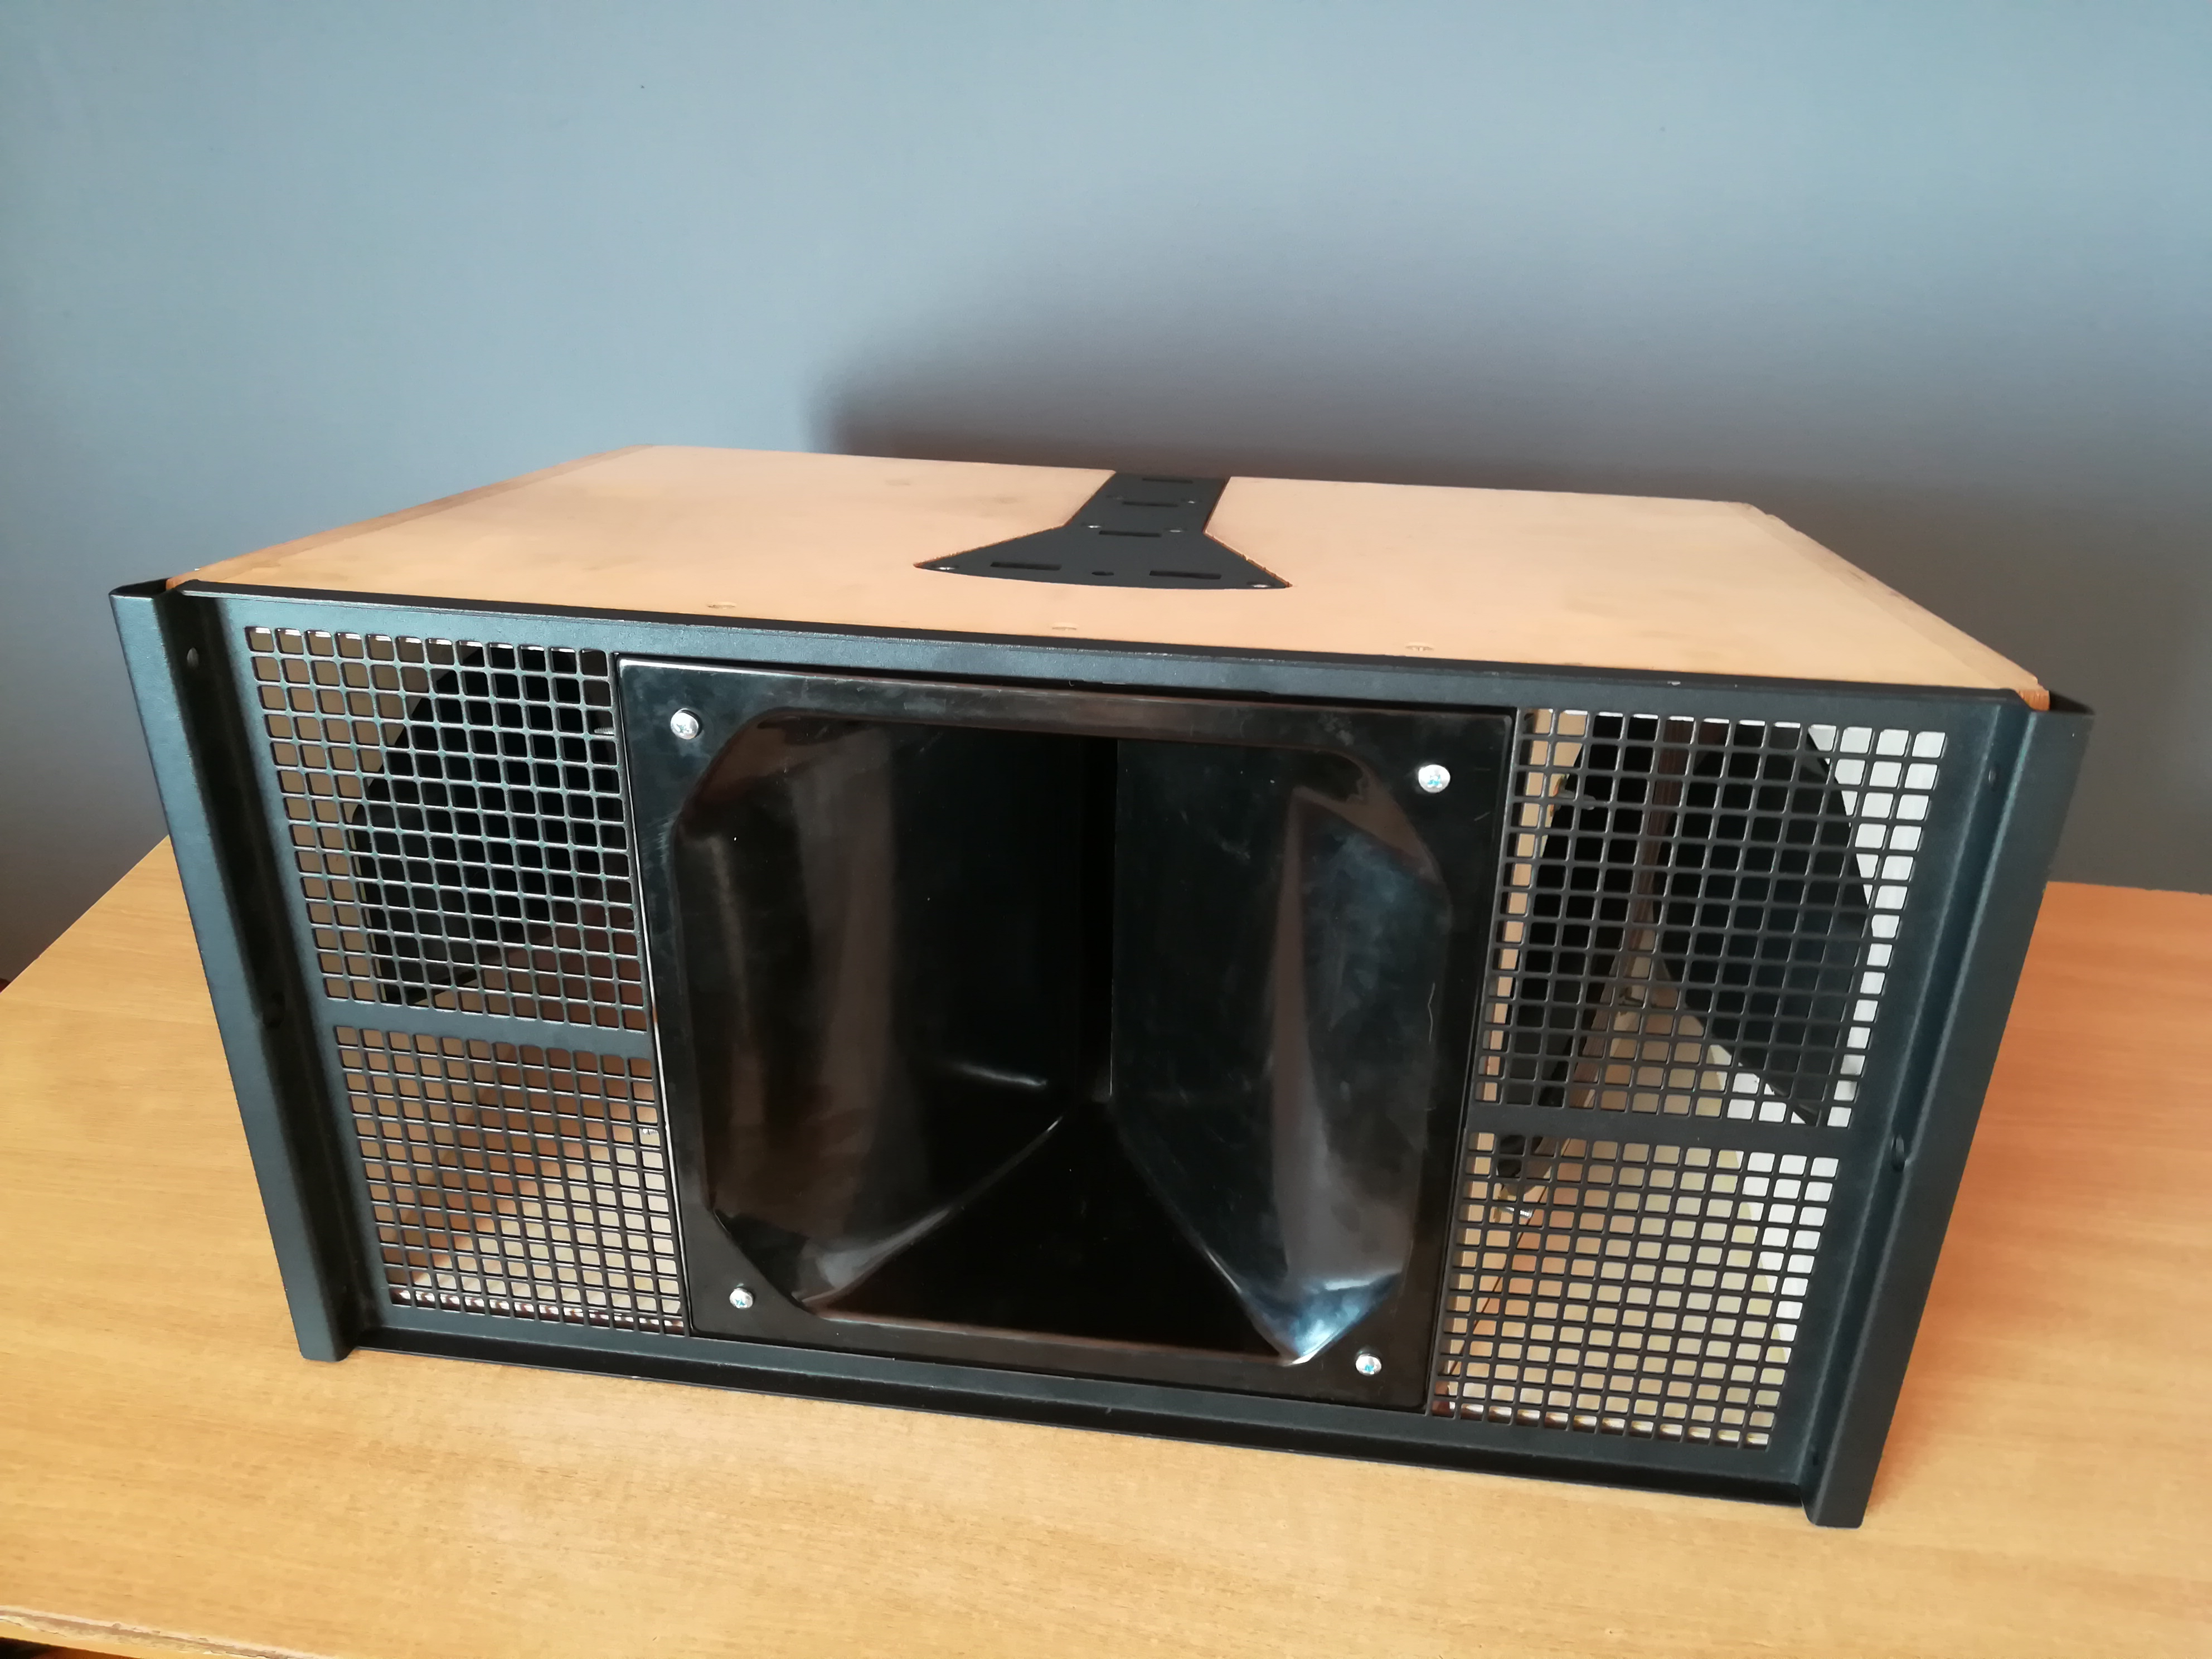
\includegraphics[width=.8\textwidth]{zdjecie.jpg}
		\caption{Badany zestaw głośnikowy}
		\label{r:zdjecie}
	\end{figure}
	
	\begin{figure}[!ht]
		\centering
		\adjincludegraphics[width=.9\textwidth,trim={{.1\width} {.25\height} {.17\width} {.12\height}},clip]{render_z_otworami_bez_tekstury.pdf}\\
% 		\setlength{\unitlength}{1cm}
% 		\begin{picture}(0,0)
% 			\thicklines
% 			\put(-2,3){\line(-1,1)}
% 			\put(-3){1}
% % 			\put(-6,2){\line}
% % 			\put(){2}
% % 			\put(-6,2){\line}
% % 			\put(){3}
% 		\end{picture}
		\caption{Przekrój modelu badanego zestawu głośnikowego w~płaszczyźnie poziomej; 1~--~głośniki niskotonowe, 2~--~zespół głośnika wysoktonowego, 3~--~otwór \textit{bass-reflex}}
		\label{r:przekroj}
	\end{figure}
	
	\subsection{Modyfikacja obudowy}
	
	% 		W~celu określenia wpływu konstrukcji obudowy na parametry zestawu głośnikowego zastosowano wybrane rodzaje jej modyfikacji. Wybrano modyfikacje możliwe do faktycznego zastosowania, a~jednocześnie takie, które nie wymagają nieodwracalnej ingerencji w~obudowę.
	W~celu określenia wpływu konstrukcji obudowy na parametry zestawu głośnikowego zastosowano modyfikację polegającą na zaślepieniu otworów \textit{bass-reflex}. Taka zmiana znacząco zmienia charakter obudowy (na zamkniętą), a~jednocześnie nie wymaga nieodwracalnej ingerencji w~jej konstrukcję.
	
	Oprócz modyfikacji obudowy, zmieniano także liczbę zamontowanych w~niej głośników, aby lepiej zbadać ich wzajemny wpływ. Wszystkie konfiguracje pomiarowe opisano w~tabeli~\ref{t:obudowa}.
	
	\begin{table}[!ht]
		\centering
		\caption{Opis konfiguracji obudowy i~głośników wykorzystanych podczas pomiarów}
		\label{t:obudowa}
		\begin{tabular}{|c|c|m{.6\textwidth}|}
			\hline
			\textbf{L.p.} & \makecell{\textbf{Oznaczenie}\\\textbf{(na wykresach)}} & \centering\textbf{Opis} \tabularnewline\hline
			1. & Podstawowa & Obudowa w~podstawowej wersji (opisanej w~części~\ref{ss:opis}), z~otworami, bez wypełnienia \\\hline
			2. & Zaślepiona & Ćwierćkoliste otwory zaślepione elementami ze sklejki o~grubości \SI{6,4}{\milli\metre}, przyklejonymi do ścianki, w~której zamocowany jest głośnik niskotonowy\\\hline
			\hline
			3. & Jeden głośnik & Jeden głośnik niskotonowy zamocowany w~obudowie, otwór na drugi zaślepiony kołem ze sklejki; zamocowany zespół głośnika wysokotonowego \\\hline
			4. & Dwa głośniki & Obydwa głośniki niskotonowe oraz zespół głośnika wysokotonowego zamocowane w~obudowie\\\hline
		\end{tabular}
	\end{table}
	
	\section{Metodyka pomiarów}
	
	W~celu możliwie dokładnego zbadania parametrów zestawu, ze szczególnym uwzględnieniem obudowy, zaplanowano szereg pomiarów: impedancji elektrycznej głośnika w~odgrodzie z~wyznaczeniem parametrów Thiele-Smalla, charakterystyki skuteczności, charakterystyk kierunkowości oraz pomiar drgań obudowy przy pomocy wibrometru laserowego.
	
	Ze względu na zaobserwowane znaczące rozbieżności między wynikami uzyskanymi dla głośników niskotonowych, a~parametrami podanymi przez producenta w~karcie katalogowej, zdecydowano się na wykonanie dodatkowych pomiarów, uwzględniających zużycie głośnika.
	
	Metodyka pomiarów opierała się na wytycznych zawartych w~normie EN~60268-5~\cite{norma}. Natężenie prądu elektrycznego i~napięcie elektryczne tam, gdzie to było konieczne, monitorowano przy pomocy multimetrów Tektronix DMM~4040 oraz DMM~4050.
	
	\subsection{Impedancja elektryczna i parametry Thiele-Smalla}
	
	Pomiary wykonano przy pomocy systemu Brüel\&Kjær Pulse, pozwalającego na pomiar charakterystyki impedancji oraz wyznaczenie na tej podstawie parametrów Thiele-Smalla.
	
	Istnieją dwie metody pomiaru tych parametrów: metoda dodanej masy oraz metoda dodanej objętości. Ze względów praktycznych zdecydowano się na wykonywanie większości pomiarów metodą dodanej masy, dla porównania wykonano też jeden pomiar metodą dodanej objętości.
	
	Procedura pomiaru metodą dodanej masy wyglądała następująco: wykonano pomiar charakterystyki impedancji głośnika, a~następnie do membrany dodano masę $m=\,$\SI{10}{\gram} i~wykonano kolejny pomiar. Na podstawie porównania dwóch charakterystyk impedancji, za pomocą dedykowanego oprogramowania Pulse Thiele Small Parameters Calculation BZ-5604 wyznaczano parametry Thiele-Smalla~\cite{BK_pulse_TS}, opisane w~tabeli~\ref{t:TS_opis}.
	
	Opracowano także skrypt w~środowisku Matlab wyznaczający te parametry z~zarejestrowanych charakterystyk impedancji na podstawie~\cite{dobrucki}; działanie skryptu zostało zweryfikowane w~oparciu o~parametry wyznaczone w narzędziu B\&K Pulse.
	
	\begin{table}[!ht]
		\centering
		\caption{Opis parametrów Thiele-Smalla, za~\cite{BK_pulse_TS}~i~\cite{dobrucki}}
		\label{t:TS_opis}
		\begin{tabular}{|l|c|c|}
			\hline
			\textbf{Oznaczenie} & \textbf{Jednostka} & \textbf{Opis parametru}\\\hline\hline
			\multicolumn{3}{|c|}{Parametry wyznaczane z pojedynczego pomiaru} \\\hline\hline
			$F_s$ & \si{\hertz} & Częstotliwość rezonansowa \\\hline
			$Z_{max}$ & \si{\ohm} & Impedancja w~rezonansie \\\hline
			$R_e$ & \si{\ohm} & Rezystancja dla napięcia stałego \\\hline
			\gape{$r_0=\frac{Z_{max}}{R_e}$} & --- & Stosunek impedancji cewki do rezystancji \\\hline
			$S$ & \% & \makecell{Symetria rezonansu, wyznacznik wiarygodności\\obliczonych parametrów -- powinna wynosić najwyżej 3,5\%} \\\hline
			\hline
			$Q_{ms}$ & --- & Dobroć mechaniczna \\\hline
			$Q_{es}$ & --- & Dobroć elektryczna \\\hline
			\gape{$Q_{ts}=\frac{Q_{ms}\cdot Q_{es}}{Q_{ms}+Q_{es}}$} & --- & Dobroć całkowita \\\hline
			\hline
			\multicolumn{3}{|c|}{Parametry wyznaczane z dwóch pomiarów (samej membrany i z dodaną masą)} \\\hline\hline
			$V_{as}$ & \si{\deci\metre\cubed} & Równoważna objętość podatności głośnika \\\hline
			$M_{ms}$ & \si{\gram} & Masa mechaniczna membrany \\\hline
			$C_{ms}$ & \si[per-mode=symbol]{\metre\per\newton} & Podatność mechaniczna zawieszenia \\\hline
			$R_{ms}$ & \si[per-mode=symbol]{\metre\per\newton} & Rezystancja mechaniczna głośnika \\\hline
			\hline
			$M_{as}$ & \si[per-mode=symbol]{\kilo\gram\per\metre\tothe{4}} & Masa akustyczna membrany \\\hline
			$C_{as}$ & \si[per-mode=symbol]{\metre\tothe{5}\per\newton} & Podatność akustyczna zawieszenia \\\hline
			$R_{as}$ & \si[per-mode=symbol]{\newton\s\per\metre\tothe{5}} & Rezystancja akustyczna głośnika \\\hline
			\hline
			$\eta_0$ & \% & Sprawność głośnika \\\hline
			$Bl$ & \si{\tesla\metre} & \makecell{Współczynnik przetwarzania elektromechanicznego\\(indeks siły)} \\\hline
			$L_{e}$ & \si{\henry} & Indukcyjność cewki dla częstotliwości \SI{1}{\kilo\hertz} \\\hline
		\end{tabular}
	\end{table}
	
	
	Pomiar wykonano z~użyciem sygnału sinusoidalnego z~krokiem $1/48$~oktawy w~zakresie \range{20}{8000}~\si{\hertz}. Zmierzono impedancję głośnika niskotonowego w~odgrodzie oraz głośników w~obudowie z~zastosowanymi różnymi modyfikacjami.
	
	Ze względu na rozbieżności między parametrami katalogowymi a~rzeczywistymi oraz dla różnych egzemplarzy tego samego modelu głośnika~\cite{aes_roznice}, wykonano pomiary pozwalające na porównanie obu wykorzystywanych egzemplarzy oraz sprawdzenie, jak zmieniają się parametry głośnika podczas jego eksploatacji. Pomiary wykonano na fabrycznie nowym przetworniku oraz na tym samym egzemplarzu poddanym procesowi zużycia poprzez dostarczenie w dwóch etapach sygnału szumu różowego: o~mocy \SI{40}{\watt} przez czas \SI{2}{\hour} w~pierwszym etapie i~\SI{60}{\watt} przez czas \SI{10}{\min} w drugim etapie.
	
	\subsection{Charakterystyka skuteczności i~skuteczność}
	
	Do pomiarów wykorzystano analizator SVAN 912E; głośnik pobudzano szumem różowym z~generatora o~wartości skutecznej \SI{1}{\watt}. Analizę prowadzono w~odległości \SI{2}{\metre} w~pasmach $1/3$-oktawowych w~zakresie \range{50}{5000}~\si{\hertz}.
	
	W celu weryfikacji skuteczności podawanej przez producenta wykonano też pomiar poziomu dźwięku $L_{eq}$ przy użyciu tego samego analizatora. 
	
	\subsection{Charakterystyki kierunkowości}
	
	% 			Wykonano dwie serie pomiarów, dla głośnika wysoko- i~niskotonowego. W~pierwszej serii zmierzono głośniki w~obudowie bez wypełnienia, w~drugiej -- wypełnione materiałem dźwiękochłonnym.
	
	Pomiar charakterystyki kierunkowości odbywał się w~komorze bezechowej przy użyciu stolika obrotowego, na którym umieszczony był zestaw głośnikowy. W~osi akustycznej mierzonego głośnika ustawiono mikrofon GRAS 46AE; następnie głośnik obracano z~krokiem \SI{10}{\degree}, każdorazowo zatrzymując i~wykonując pomiar trwający \SI{3}{\s}. Sygnałem podawanym na głośnik był szum różowy, pomiar wykonano w~pasmach $1/6$~oktawy, w~zakresie \range{40}{20000}~\si{\hertz}.
	
	\subsection{Drgania obudowy}
	
	Pomiar drgań obudowy miał na celu sprawdzenie, w~jakim stopniu charakterystyka częstotliwościowa zestawu jest związana z~właściwościami obudowy. Badany zestaw głośnikowy umieszczono w~komorze bezechowej; w~wybranych punktach (por. rys.~\ref{r:wibro_pkt}) naklejono taśmę odblaskową, na którą padała wiązka lasera; zastosowanie taśmy było niezbędne dla uzyskania odpowiedniego odbicia światła od badanych powierzchni. %Wibrometr umieszczono w~odpowiedniej odległości, tak aby uniknąć przesterowania sygnału. 
	Sygnałem pomiarowym był szum różowy, rejestrowano jednocześnie przebieg drgań wibrometrem oraz sygnał akustyczny dwoma mikrofonami: jednym umieszczonym blisko bieżącego punktu pomiarowego (\range{6}{10}~\si{\cm} od punktu pomiaru -- rys.~\ref{r:wibro_zdjecie}), a~drugim w~odległości~\SI{2}{\metre}. Wibrometr umieszczono poza przestrzenią komory celem zapewnienia jego stabilnego usadowienia.
	
	\begin{figure}[!ht]
		\centering
		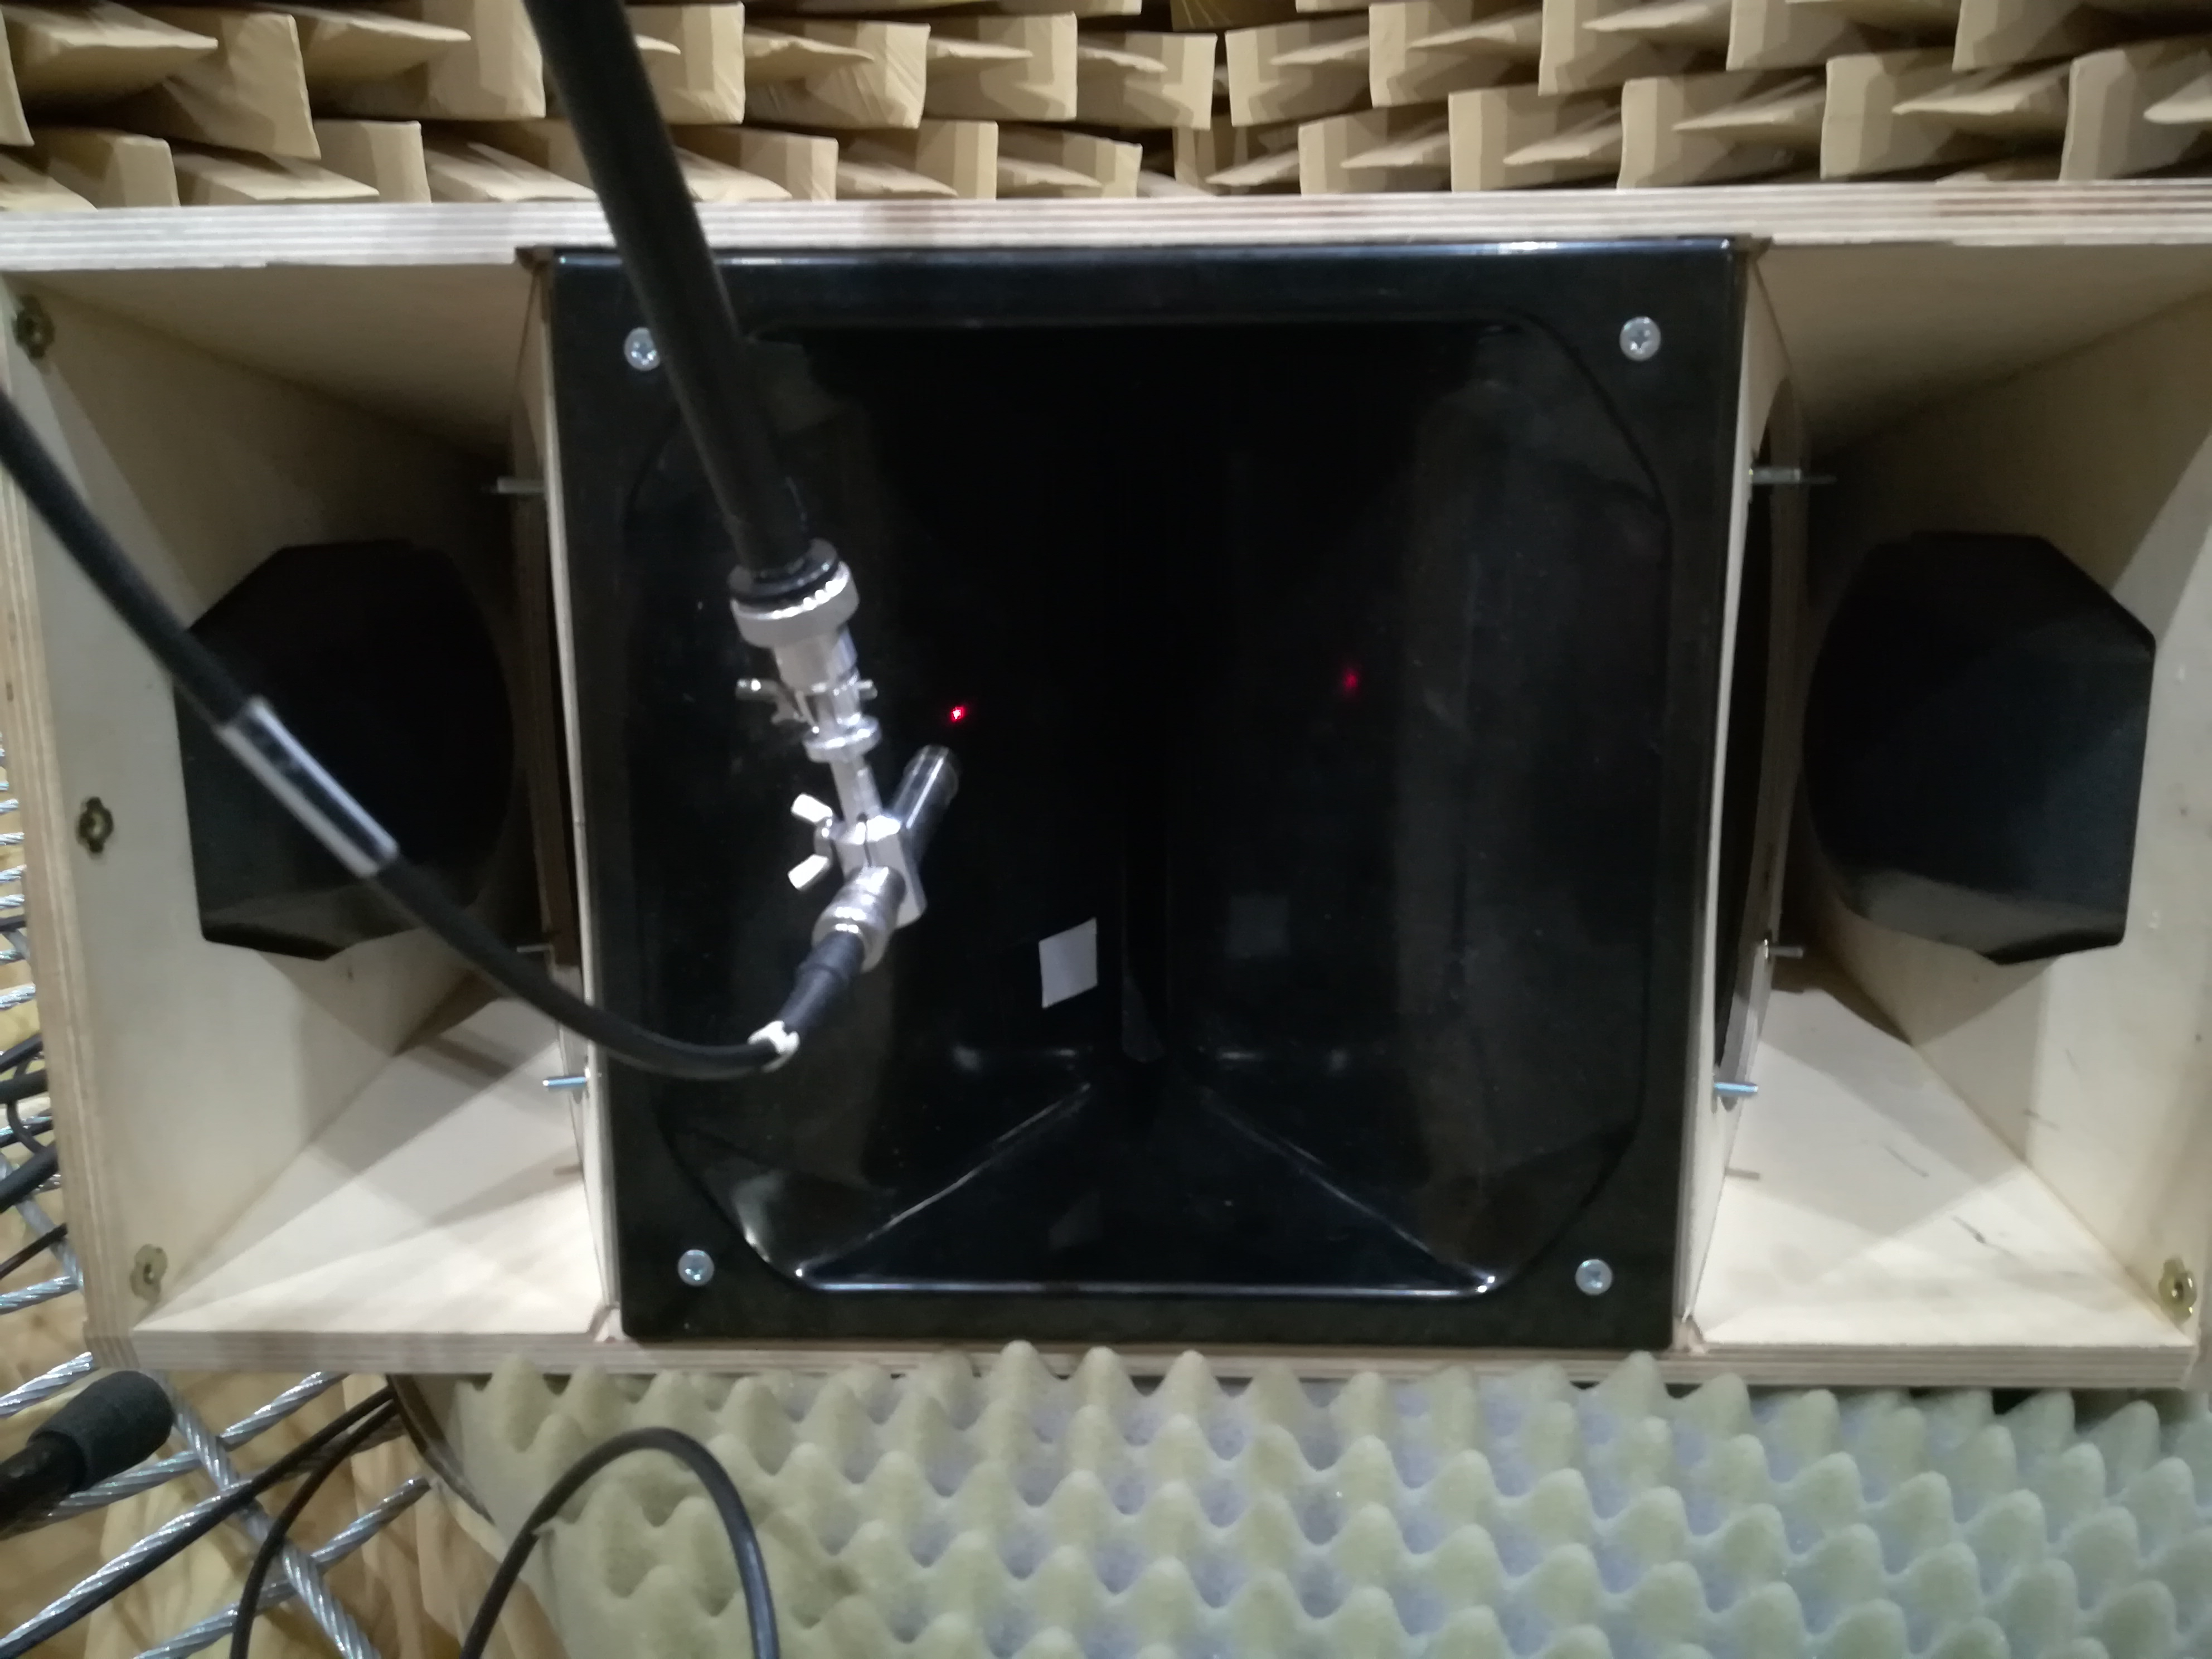
\includegraphics[width=.7\textwidth]{zdjecie_wibro.jpg}
		\caption{Fotografia wykonana podczas przygotowań do pomiaru z~użyciem wibrometru}
		\label{r:wibro_zdjecie}
	\end{figure}
	
	
	\section{Modelowanie}
	
	\subsection{Wprowadzenie}
	
	Dzięki stworzeniu modelu komputerowego możliwe jest łatwe i~niewymagające wysokich kosztów testowanie różnych rozwiązań metodami numerycznymi. Takie rozwiązanie pozwala również na dużo prostszą obserwację zjawisk akustycznych i~mechanicznych zachodzących w~konstrukcji i~nie wymaga użycia zaplecza technicznego takiego jak np. komora bezechowa. 
	
	Jednak tworzenie skomplikowanych modeli wykorzystujących sprzężenie pomiędzy domeną mechaniczną opisującą zachowanie membrany i~zawieszenia głośnika, a~domeną akustyczną opisującą propagację dźwięku w~powietrzu, wymaga poznania właściwości materiałów, z których zbudowane są wszystkie elementy. Parametry materiałowe, takie jak moduł Younga, współczynnik Poissona, czy gęstość, ciężko jest zmierzyć dla każdego elementu modelu, a~jednocześnie odpowiadają za jego właściwości mechaniczne, a~co za tym idzie -- pośrednio -- akustyczne. W~praktyce zazwyczaj wykorzystuje się jako bazę właściwości materiałów dostępne w~literaturze~\cite{modelowanie}, a~następnie przeprowadza strojenie modelu -- dla znanego przypadku wykonuje się symulacje, zmieniając parametry tak, aby wyniki otrzymane w~modelu komputerowym były jak najbardziej zbliżone do wyników pomiaru.
	
	Dodatkowo problematyczne staje się stworzenie geometrii, dla której możliwe byłoby wygenerowanie siatki elementów, przy jednoczesnym odwzorowaniu kształtu w~sposób zapewniający rzeczywiste zachowanie elementów modelu. Na taki problem natknęli się autorzy przy tworzeniu kształtu zawieszenia, co można zaobserwować na rysunku~\ref{r:zawieszenie}, przedstawiającym przemieszczenia w~symulacji dla częstotliwości \SI{50}{\hertz} -- widoczne jest przemieszczenie membrany w~dół i~przemieszczenie zawieszenia w~sposób nieadekwatny do ruchu membrany.
	Związany z~tym jest problem rozmiarów elementów siatki, który z~kolei wpływa na czas obliczeń modelu. Dla wysokich częstotliwości i dużych modeli ilość węzłów staje się na tyle duża, że czas obliczeń nawet na komputerach o~dużej mocy obliczeniowej jest bardzo długi, przez co model jest bezużyteczny.
	
	\begin{figure}[!ht]
		\centering
		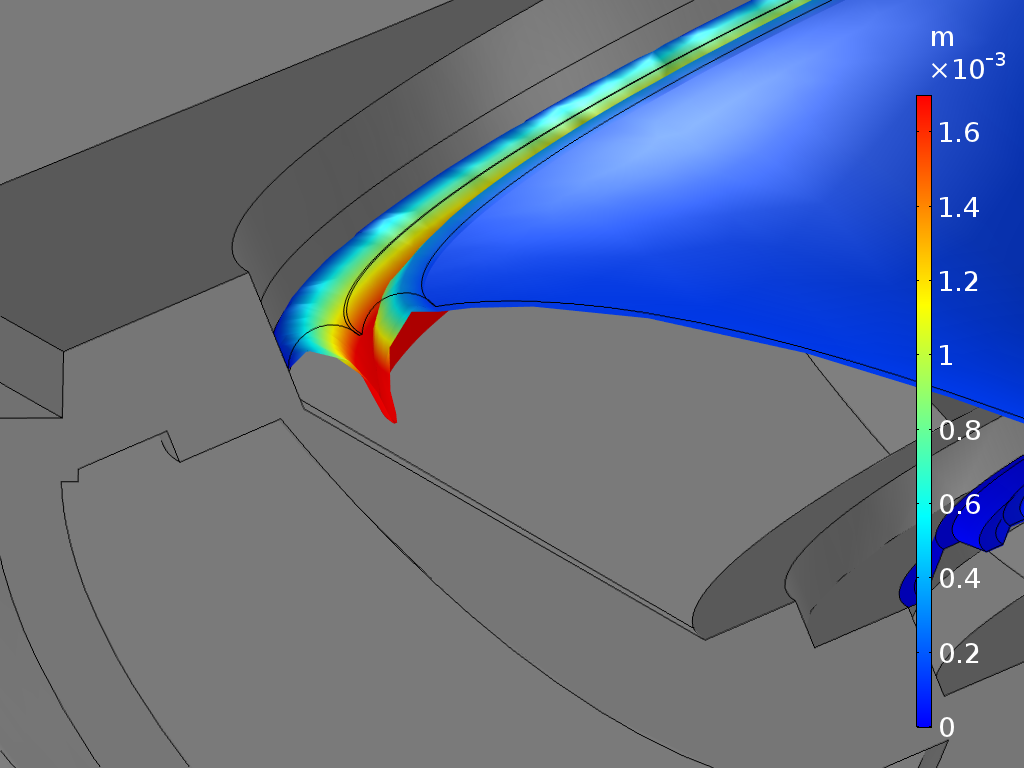
\includegraphics[width=.7\textwidth]{disp_factor5_f50_02.png}
		\caption{Przemieszczenia górnego zawieszenia w~symulacji dla częstotliwości \SI{50}{\hertz}}
		\label{r:zawieszenie}
	\end{figure}
	
	\subsection{Wykonany model}
	
	Aby zyskać możliwość wprowadzania modyfikacji obudowy, zdecydowano się na wykonanie modelu badanego zestawu. Geometrię przygotowano w~programie Autodesk Inventor; obliczenia prowadzono za pomocą metody elementów skończonych (MES) w~środowisku Comsol Multiphysics, z~wykorzystaniem modułu akustycznego i~mechanicznego. Elementowi cewki przypisywano wartość siły obliczonej na podstawie zależności~\eqref{eq:sila}:
	
	\begin{equation}
	F_e=\frac{BlV_0}{Z_b}-\nu\frac{(Bl)^2}{Z_b} \quad, \label{eq:sila}
	\end{equation}
	
	\noindent gdzie $Bl$ jest indeksem siły (por. tab.~\ref{t:TS_opis}), $V_0$ napięciem zasilania głośnika, $Z_b$ impedancją zablokowanej cewki, a~$\nu$ prędkością cewki. 
	
	W~oparciu o~te dane program wyznacza przemieszczenia membrany, które dzięki sprzężeniu pomiędzy modułem akustycznym i~mechanicznym pozwalają na wyznaczenie rozkładu ciśnienia akustycznego w~powietrzu.
	
	Ze względu na brak możliwości zidentyfikowania parametrów materiałów użytych przez producenta głośników, zdecydowano się na próbę skorygowania parametrów zaczerpniętych z~literatury \cite{modelowanie} poprzez dostrojenie modelu. Wszystko to w~celu najlepszego odzwierciedlenia właściwości badanego zestawu. Proces ten nie został jeszcze zakończony.
	
	
	\section{Analiza wyników}
	
	\subsection{Pomiary impedancji}
	
	%Z~przyczyn technicznych parametry T-S dla tego pomiaru zostały obliczone na podstawie dostępnych materiałów (\cite{dobrucki},), a~nie wyznaczone przy pomocy systemu Pulse.
	Parametry Thiele-Smalla zostały wyznaczone z~zarejestrowanych krzywych impedancji przy pomocy skryptu w~środowisku Matlab na podstawie~\cite{dobrucki}. Następnie działanie skryptu zostało zweryfikowane w~oparciu o~parametry wyznaczone w~narzędziu B\&K Pulse. 
	
	W~wynikach wszystkich pomiarów wykonanych w~odgrodzie widoczny jest jej wpływ -- charakterystyka załamuje się w~okolicach częstotliwości \SI{54}{\hertz}. Prawdopodobnie związane jest to z~rezonansem płyty, występującym ze względu na jej skończone wymiary.
	
	Na rysunku \ref{r:metody} przedstawione zostały przebiegi impedancji w~funkcji częstotliwości zmierzone dla obu metod. Widoczne jest przesunięcie częstotliwości rezonansowej w~dół po dodaniu masy i~w~górę po dodaniu objętości, natomiast w~tabeli~\ref{t:TS_metody} przedstawiono parametry Thiele-Smalla uzyskane obiema metodami (kolumna 4~i~5). Przyjmują one podobne wartości dla obu metod, nie widać też znaczących różnic w~symetrii $S$ -- dla obu pomiarów parametr ten jest wystarczająco niski. 
	
	Porównano także wyniki pomiaru metodą dodanej masy dla tego samego głośnika po pierwszym etapie: masa wynosiła \SI{5}{\gram} i~\SI{10}{\gram}. Wyniki wskazują, że wartość \SI{5}{\gram} może być zbyt mała -- różnica częstotliwości rezonansowych nie jest wystarczająco duża, a~co za tym idzie, wyznaczone parametry nie są wiarygodne, co potwierdza zbyt duża wartość symetrii $S$ (powyżej \SI{3,5}{\%}).
	
	\begin{figure}[!ht]
		\centering
		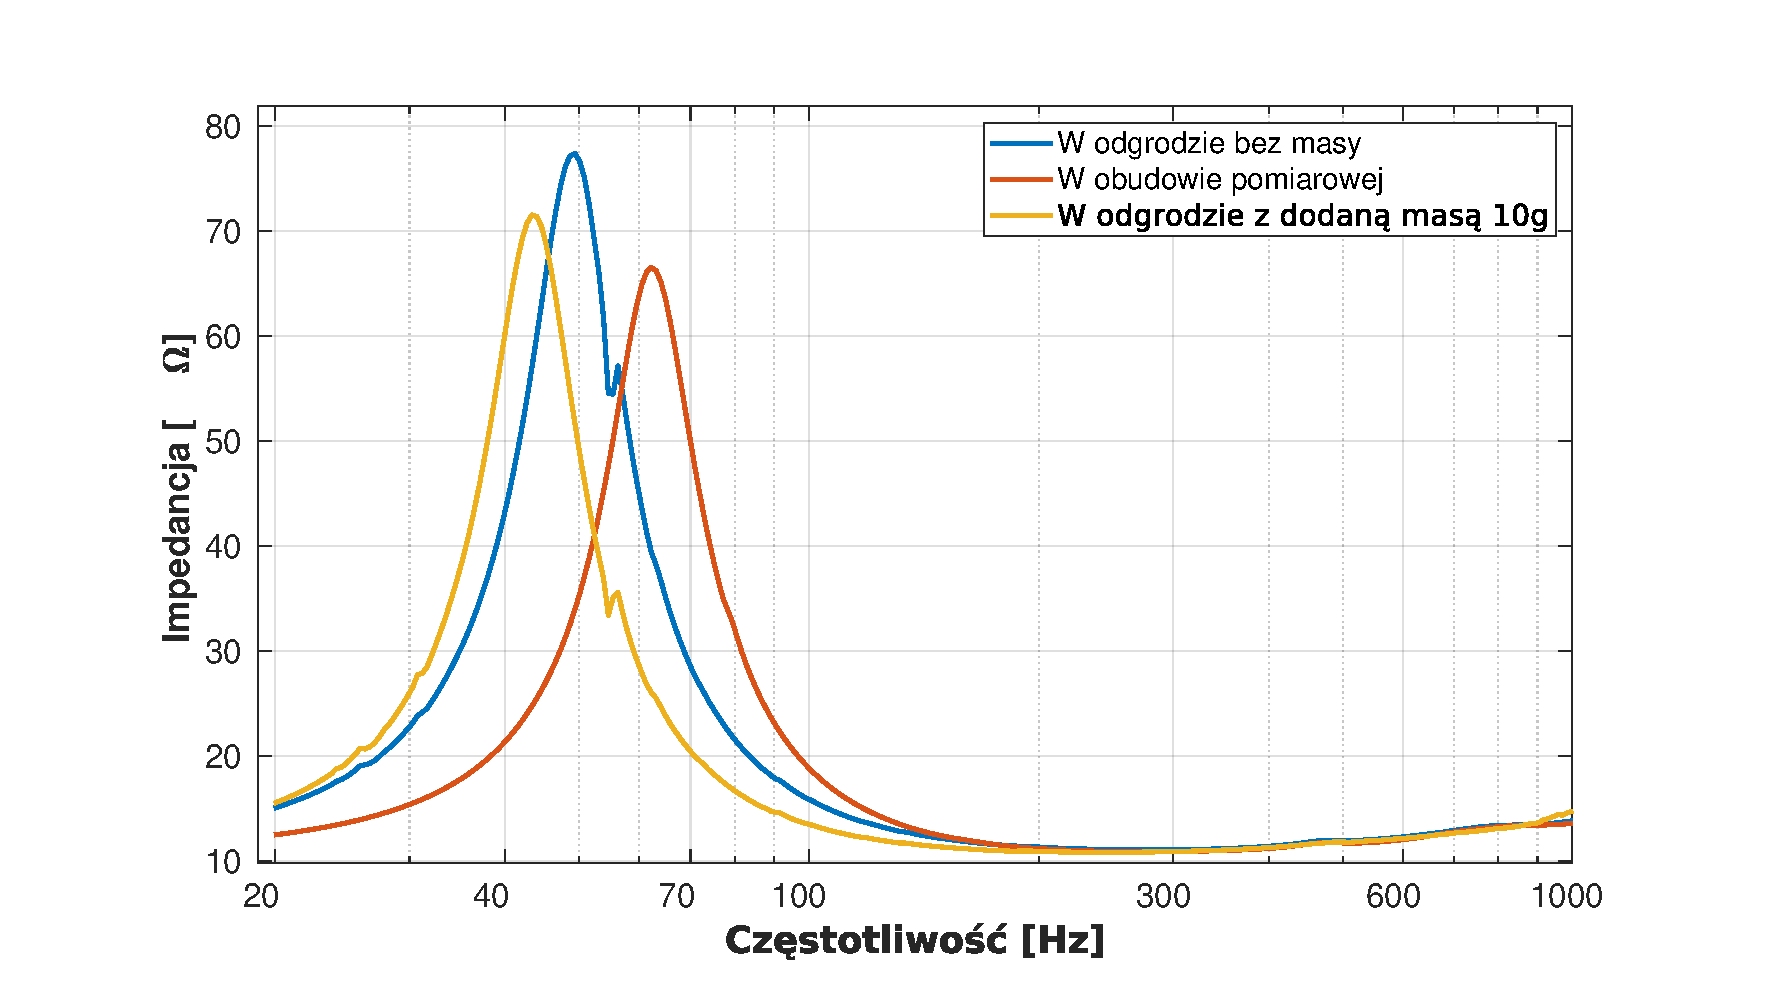
\includegraphics[width=.8\textwidth,trim={2cm .5cm 2cm 1cm},clip]{metody_2glosnik.pdf}
		\caption{Charakterystyki impedancji głośnika w~odgrodzie oraz głośnika przy pomiarze każdą z~metod (dodanej masy i~dodanej objętości) po drugim etapie zużycia}
		\label{r:metody}
	\end{figure}
	
	\begin{table}[!ht]
		\centering
		\caption{Porównanie metod pomiaru parametrów Thiele-Smalla: dodanej masy oraz objętości na etapie~2, oraz różnych wartości masy na etapie~1}
		\label{t:TS_metody}
		\boldmath
		\begin{tabular}{|l|}
			\hline
			\multirow{2}{*}{\textbf{Parametr}} 	\\
			\\\hline
			\hline                              							
			$F_s$ [\si{\hertz}] \\\hline
			$Z_{max}$ [\si{\ohm}] \\\hline
			$R_e$ [\si{\ohm}] \\\hline
			$r_0$ \\\hline
			$S$ [\%]\\\hline
			\hline                              							
			$Q_{ms}$ 	\\\hline
			$Q_{es}$ \\\hline	
			$Q_{ts}$ \\\hline
			\hline                                                  		
			$V_{as}$ [\si{\deci\metre\cubed}] \\\hline
			$M_{ms}$ [\si{\gram}] 	\\\hline
			$C_{ms}$ [\si[per-mode=symbol]{\metre\per\newton}] 	\\\hline
			$R_{ms}$ [\si[per-mode=symbol]{\metre\per\newton}] 	\\\hline
			\hline
			$M_{as}$ [\si[per-mode=symbol]{\kilo\gram\per\metre\tothe{4}}] 	\\\hline
			$C_{as}$ [\si[per-mode=symbol]{\metre\tothe{5}\per\newton}] \\\hline	
			$R_{as}$ [\si[per-mode=symbol]{\newton\s\per\metre\tothe{5}}] 	\\\hline
			\hline
			$\eta_0$ [\%] 	\\\hline
			$Bl$ [\si{\tesla\metre}]	\\\hline
			$L_{e}$ [\si{\henry}] 	\\\hline
		\end{tabular}
		\unboldmath
		~ \quad
		\begin{tabular}{|c|c|}
			\hline
			\multicolumn{2}{|c|}{\textbf{Etap 1, głośnik 1}} \\\hline
			\textbf{Masa \SI{5}{\gram}} & \textbf{Masa \SI{10}{\gram}} \\\hline
			\hline
			\num{56,5} 	& \num{57,0} 	 \\\hline
			\num{57,2} 	& \num{55,7} 	 \\\hline
			\num{10,0}  	& \num{10,0} \\\hline	
			\num{5,7}  	& \num{5,6} 	 \\\hline
			\num{4,29} 	& \num{3,35}     \\\hline
			\hline
			\num{2,7}  	& \num{2,7} 	 \\\hline
			\num{0,58} 	& \num{0,58} 	 \\\hline
			\num{0,48} 	& \num{,048} 	 \\\hline
			\hline
			\num{34,5} 	& \num{34,5} 	 \\\hline
			\num{39,1} 	& \num{38,5}     \\\hline
			\num{203e-6} 	& \num{203e-6}\\\hline
			\num{5,1} 	& \num{5,2}  	  \\\hline
			\hline
			\num{32,6} 	& \num{32,1}      \\\hline
			\num{0,2e-6} 	& \num{0,2e-6}\\\hline
			\num{4254} 	& \num{4323} 	  \\\hline
			\hline
			\num{1,06} 	& \num{1,07} 	  \\\hline
			\num{15,5} 	& \num{15,4} 	  \\\hline
			\num{890e-6} 	& \num{880e-6}\\\hline
		\end{tabular}
		~ \quad
		\begin{tabular}{|c|c|}
			\hline
			\multicolumn{2}{|c|}{\textbf{Etap 2, głośnik 2}}\\\hline
			\textbf{Masa \SI{10}{\gram}} & \textbf{Obudowa \SI{80}{\deci\metre\cubed}}\\\hline
			\hline
			\num{49,2} 	& \num{50,1} \\\hline
			\num{77,5} 	& \num{73,7} \\\hline
			\num{10,1} 	& \num{10,1} \\\hline
			\num{7,8} 	& \num{7,4}\\\hline
			\num{0,80} 	& \num{0,56}\\\hline
			\hline
			\num{3,7} 	& \num{3,5}\\\hline
			\num{0,55} 	& \num{0,55}\\\hline
			\num{0,48} 	& \num{0,48}\\\hline
			\hline
			\num{45,6} 	& \num{42,8}\\\hline
			\num{39,1} 	& \num{40,2}\\\hline
			\num{267e-6} 	& \num{251e-6}\\\hline
			\num{3,3} 	& \num{3,6}\\\hline
			\hline
			\num{32,6} 	& \num{33,5}\\\hline
			\num{0,3e-6} 	& \num{0,3e-6} \\\hline
			\num{2726} 	& \num{3011}\\\hline
			\hline
			\num{0,96} 	& \num{0,96}  \\\hline
			\num{14,9} 	& \num{15,2}\\\hline
			\num{853e-6} 	& \num{845e-6} \\\hline
		\end{tabular}
	\end{table}
	
	Wyniki pomiarów potwierdzają, że zużycie głośnika wpływa na jego parametry. Krzywe impedancji głośników w~odgrodzie po każdym etapie przedstawiono na rysunku~\ref{r:wygrzewanie}. Natomiast porównanie obu głośników na etapie~1 przedstawiono na rysunku~\ref{r:2glosniki}.
	
	W~tabeli~\ref{t:TS_karta_etapy} zestawiono wartości parametrów Thiele-Smalla na każdym etapie zużycia głośnika oraz podane w~karcie katalogowej. Należy zwrócić uwagę na fakt, że podane parametry z~karty katalogowej dotyczą głośnika o~rezystancji \SI{8}{\ohm}, podczas gdy badane egzemplarze mają rezystancję \SI{16}{\ohm}; autorom nie udało się jednak pozyskać karty katalogowej dla takiej wersji głośnika.
	
	\begin{figure}[!ht]
	\centering
	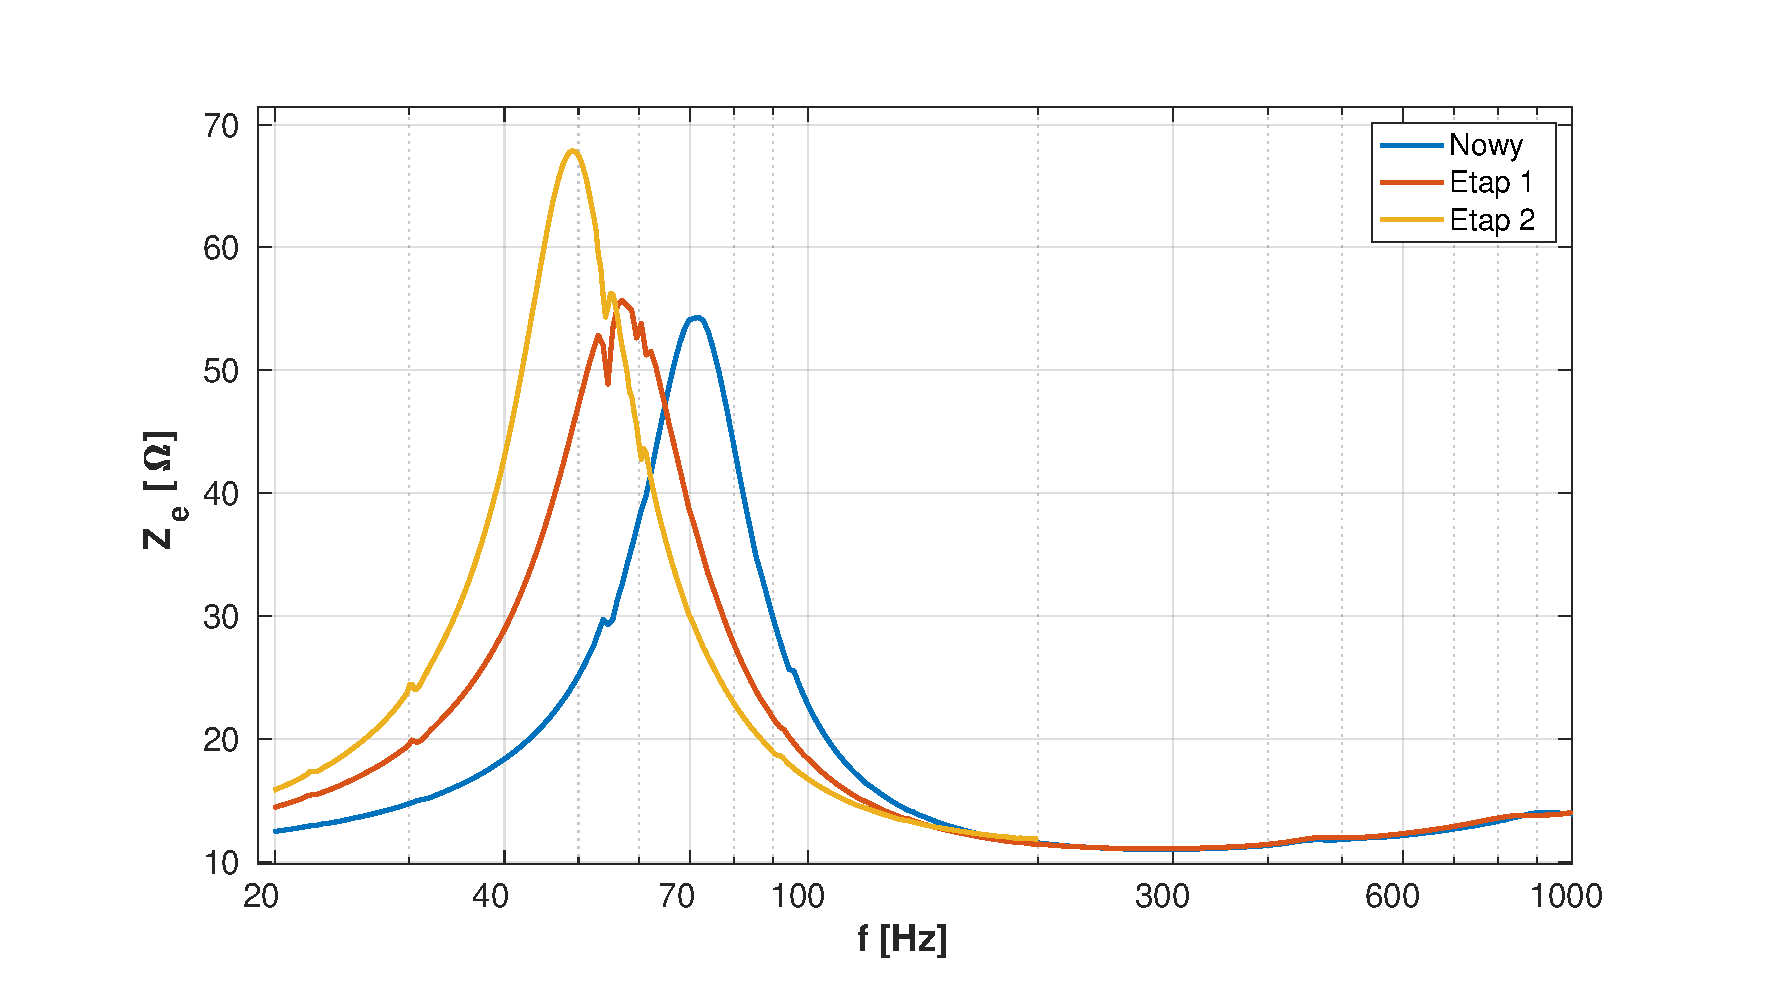
\includegraphics[width=.8\textwidth,trim={2cm .5cm 2cm 1cm},clip]{odgroda_wygrzewanie.pdf}
	\caption{Charakterystyki impedancji głośnika na różnych etapach zużycia}
	\label{r:wygrzewanie}
	\end{figure}
	
	\begin{table}[!ht]
	\centering
	\caption{Porównanie parametrów Thiele-Smalla: odczytanych z~karty katalogowej~\cite{datasheet} oraz zmierzonych metodą dodanej masy ($m=$~\SI{10}{\gram}) dla różnych etapów pracy głośnika}
	\label{t:TS_karta_etapy}
	\boldmath
	\begin{tabular}{|l|c|c|c|c|}
	\hline
	\textbf{Parametr} & \makecell{\textbf{Karta katalogowa}\\ \textbf{($R=$~\SI{8}{\ohm})}} & \textbf{Nowy} & \textbf{Etap 1} & \textbf{Etap 2} \\\hline
	\hline
	$F_s$ [\si{\hertz}] & \num{47,0}  & \num{71,5} & \num{57,0} & \num{50,7}  \\\hline
	$Z_{max}$ [\si{\ohm}] & --- & \num{54,2} & \num{55,7} & \num{64,0}  \\\hline
	$R_e$ [\si{\ohm}] & \num{6,1}  & \num{10,4} & \num{10,0} & \num{10,2}  \\\hline
	$r_0$ & ---  & \num{5,2} & \num{5,6} & \num{6,4} \\\hline
	$S$ [\%] & ---  & \num{3,44}  & \num{3,35} & \num{0,55} \\\hline
	\hline
	$Q_{ms}$ & \num{3,9}  & \num{3,3} & \num{2,7} & \num{2,8} \\\hline
	$Q_{es}$ & \num{0,4}  & \num{0,8} & \num{0,6} & \num{0,5} \\\hline
	$Q_{ts}$ & \num{0,3}  & \num{0,6} & \num{0,5} & \num{0,4} \\\hline
	\hline
	$V_{as}$ [\si{\deci\metre\cubed}] 								& \num{50,9}  & \num{23,5} & \num{34,5} & \num{41,4} \\\hline
	$M_{ms}$ [\si{\gram}] 								& \num{39,0}  & \num{36,1}  & \num{38,5} & \num{40,6} \\\hline
	$C_{ms}$ [\si[per-mode=symbol]{\metre\per\newton}] 	& \num{294e-6}  & \num{138e-6}  & \num{203e-6} & \num{243e-6} \\\hline
	$R_{ms}$ [\si[per-mode=symbol]{\metre\per\newton}] 	& \num{2,9}  & \num{5,0}  & \num{5,2} & \num{4,6} \\\hline
	\hline
	$M_{as}$ [\si[per-mode=symbol]{\kilo\gram\per\metre\tothe{4}}] 	& \num{31,8}  & \num{30,1}  & \num{32,1} & \num{33,8} \\\hline
	$C_{as}$ [\si[per-mode=symbol]{\metre\tothe{5}\per\newton}] 	& \num{0,4e-6}  & \num{0,2e-6} & \num{0,2e-6} & \num{0,3e-6}  \\\hline
	% 				$C_{as}$ [\si[per-mode=symbol]{\metre\tothe{5}\per\newton}] & \num{360e-9} & \num{165e-9} & \num{243e-9} & \num{292e-9} \\\hline
	$R_{as}$ [\si[per-mode=symbol]{\newton\s\per\metre\tothe{5}}] 	& \num{2367}  & \num{4123}  & \num{4323} & \num{3790} \\\hline
	\hline
	$\eta_0$ [\%] & \num{1,5}  & \num{1,08} & \num{1,07} & \num{1,00}   \\\hline
	$Bl$ [\si{\tesla\metre}] & \num{14,2} & \num{14,7} & \num{15,4} & \num{15,7}\\\hline
	$L_{e}$ [\si{\henry}] & \num{1e-3} & \num{1,984e-3} & \num{880e-6} & \num{911e-6} \\\hline
	\end{tabular}
	\unboldmath
	\end{table}
	
	Wyraźnie widoczny jest spadek częstotliwości rezonansowej głośnika wraz z~jego zużyciem, maleje również sprawność referencyjna $\eta_0$ oraz symetria $S$, pomiar jest więc bardziej miarodajny; rośnie natomiast indeks siły $Bl$. Porównanie obu głośników na tym samym etapie nie ukazuje wyraźnych różnic pomiędzy nimi.
	
	\begin{figure}[!ht]
	\centering
	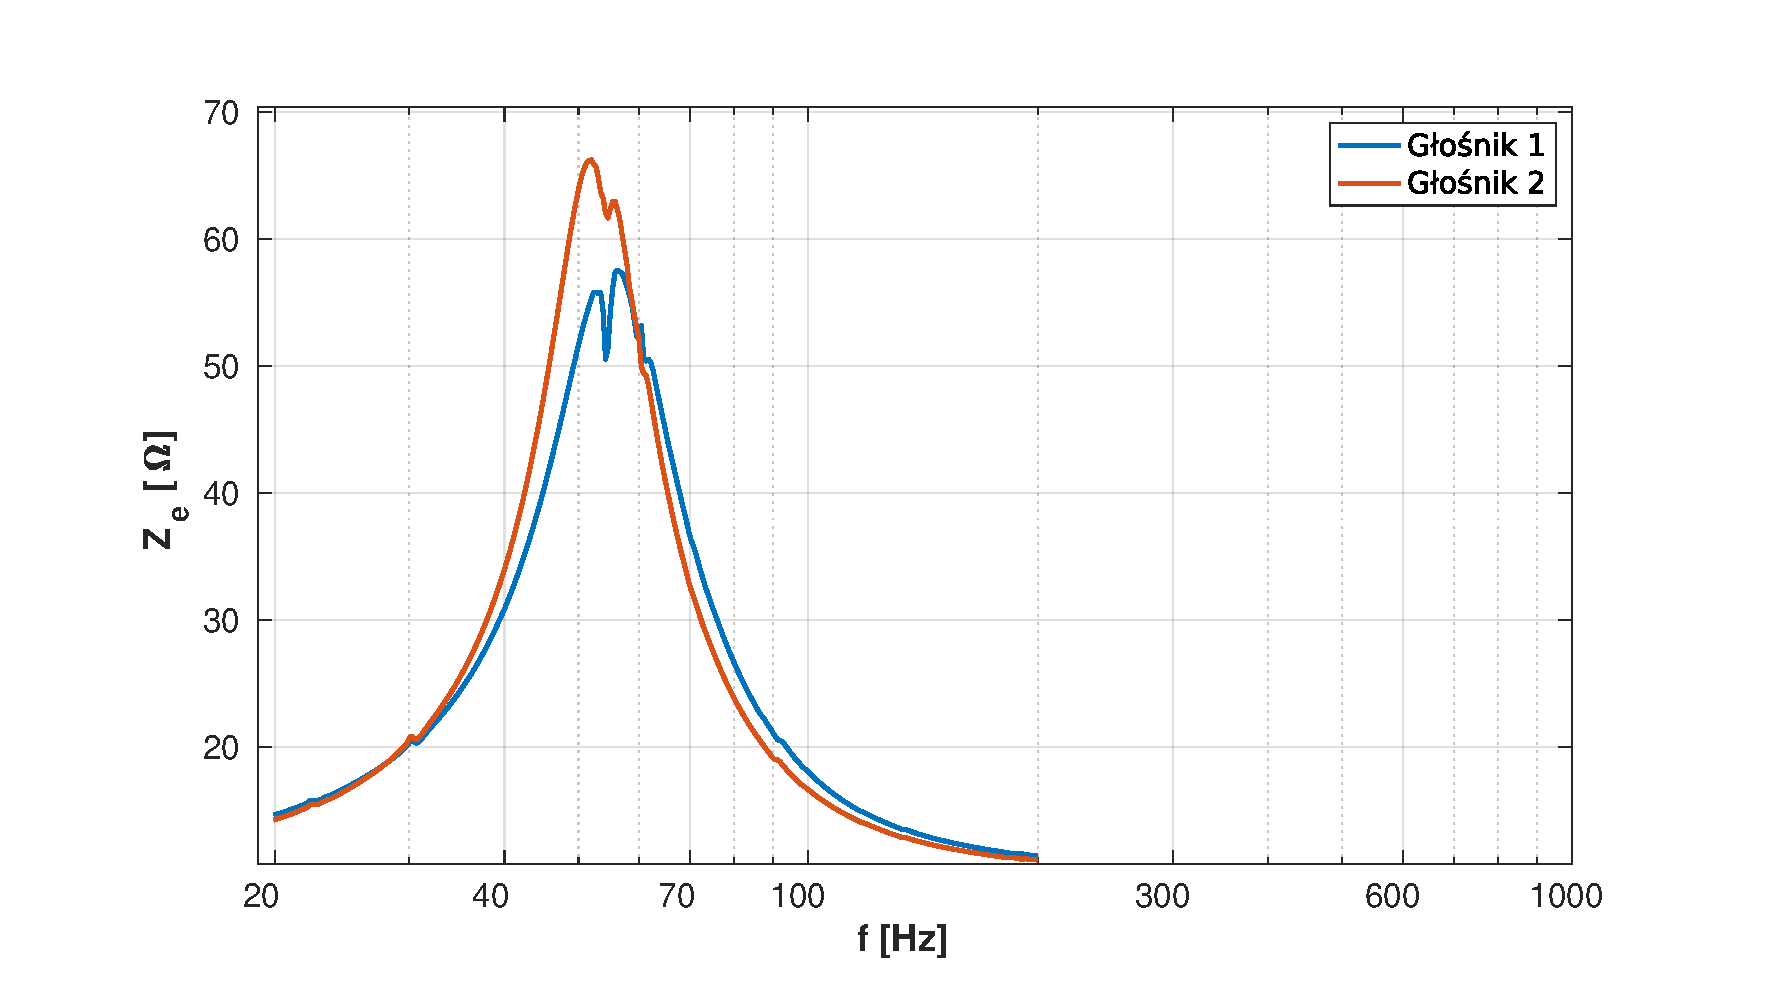
\includegraphics[width=.8\textwidth,trim={2cm .5cm 2cm 1cm},clip]{porownanie_glosnikow.pdf}
	\caption{Charakterystyki impedancji obu badanych egzemplarzy głośników w~odgrodzie po pierwszym etapie zużycia}
	\label{r:2glosniki}
	\end{figure}
	
	W~celu sprawdzenia wpływu modyfikacji obudowy na charakterystyki impedancji wykonano pomiar dla obudowy w~wariancie „podstawowym” (opisanym w~części~\ref{ss:opis}) oraz z~zaślepionymi otworami (por. tab.~\ref{t:obudowa}). Wyniki przedstawiono na rysunku~\ref{r:obudowa_otwory}. 
	Dodatkowo, dla porównania zasymulowano obie obudowy w~programie WinISD, przy czym zaślepienie otworów zostało zamodelowane jako obudowa zamknięta. Otrzymane charakterystyki znajdują się na rysunku~\ref{r:winisd}.
	
	\begin{figure}[!ht]
		\centering
		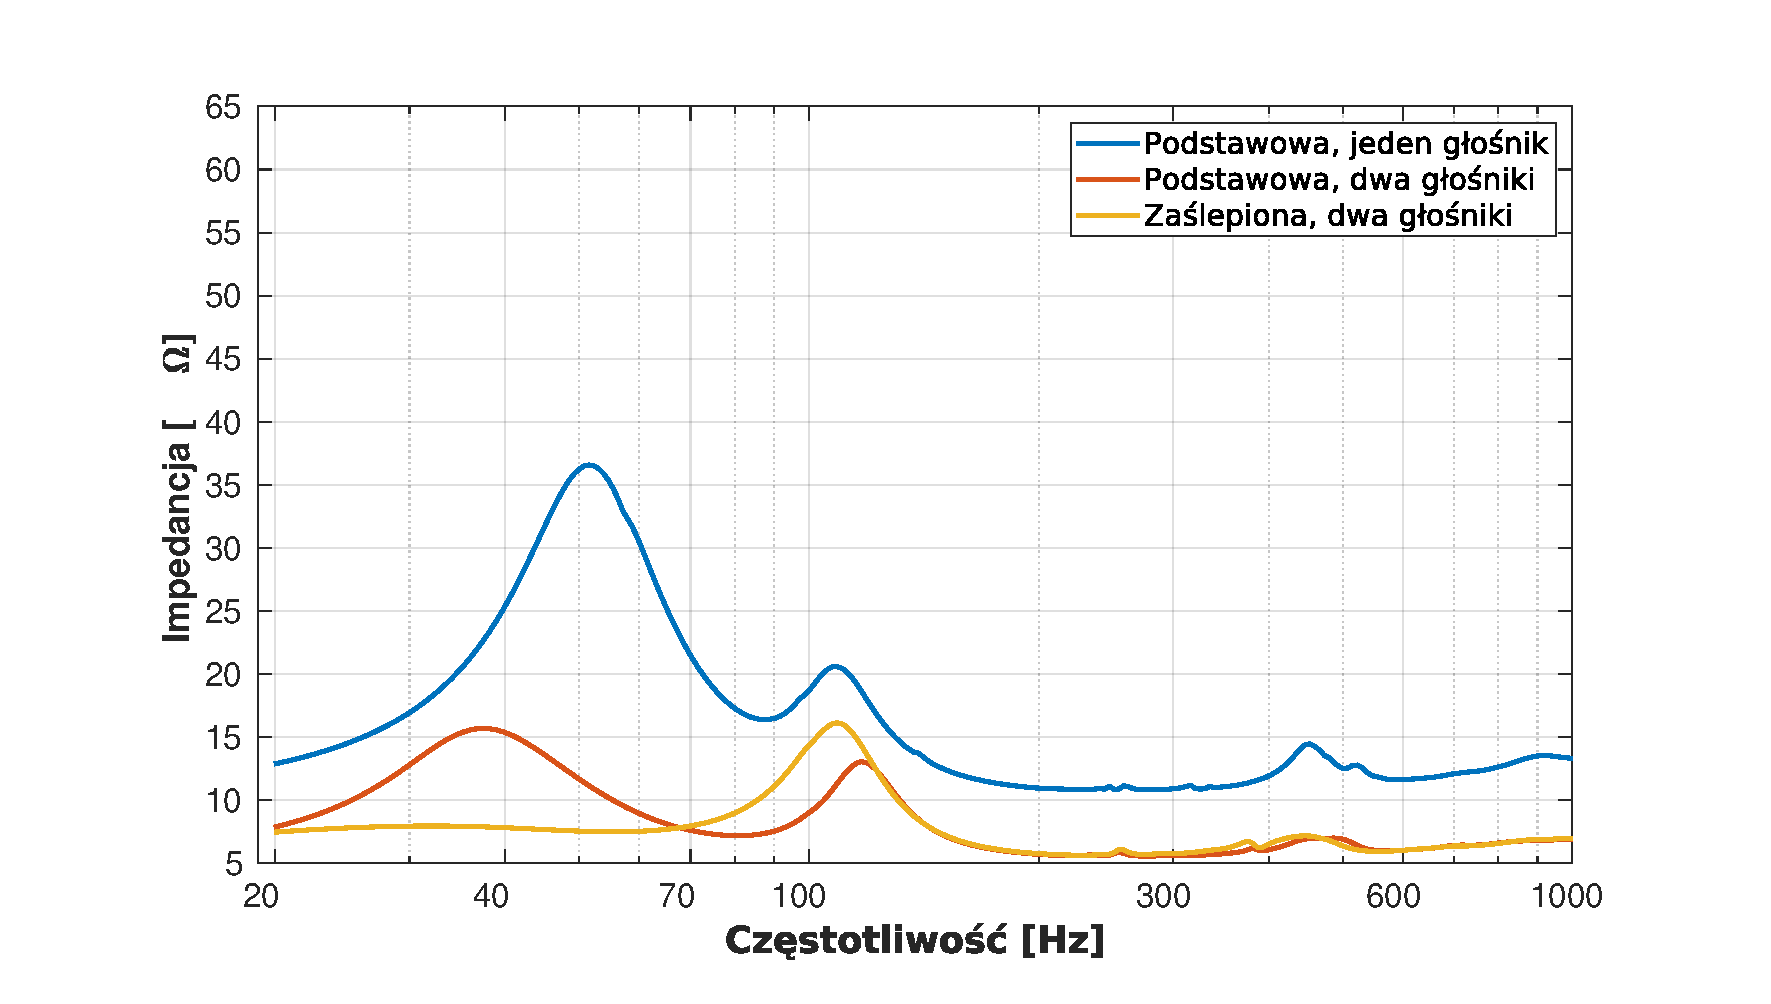
\includegraphics[width=.8\textwidth,trim={2cm .5cm 2cm 1cm},clip]{obudowa_otwory.pdf}
		\caption{Charakterystyki impedancji głośników w~obudowie z~otworami i~zaślepionej}
		\label{r:obudowa_otwory}
	\end{figure}
	
	\begin{figure}[!ht]
		\centering
		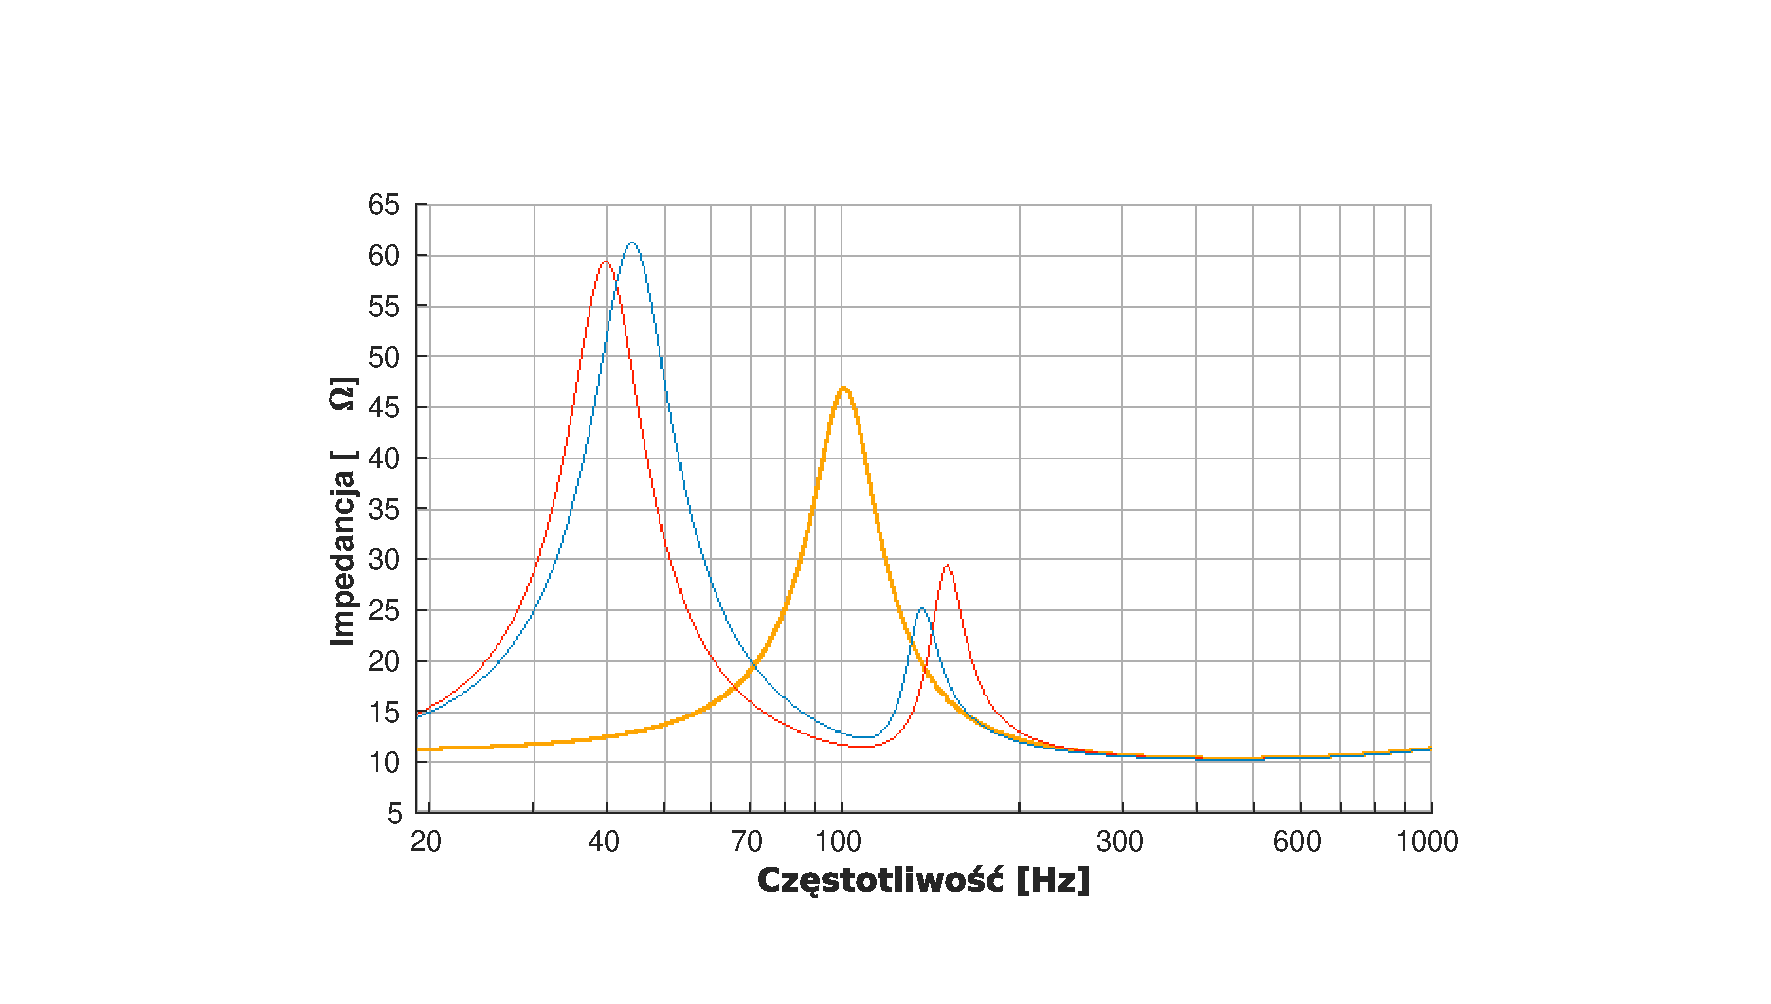
\includegraphics[width=.8\textwidth,trim={5.1cm 1.5cm 4.7cm 3cm},clip]{winisd_osie.pdf}\\
		\setlength{\unitlength}{1mm}
% 		\begin{picture}(0,0)
% 		\put(-6,2){\texttt{f [Hz]}}
% 		\put(-65,35){\rotatebox{90}{\texttt{Z$_e [\Omega]$}}}
% 		\end{picture}
		\caption{Wyniki symulacji impedancji dwóch głośników w~obudowie w~programie WinISD; \color{BrickRed}czerwony\color{Black}~--~dwa głośniki, obudowa z~otworami; \color{Dandelion}żółty\color{Black}~--~dwa głośniki, zaślepiona obudowa; \color{RoyalBlue}niebieski\color{Black}~--~jeden głośnik, obudowa z~otworami}
		\label{r:winisd}
	\end{figure}
	
	Na wykresach dla dwóch głośników w~obudowie z~otworami widoczne są dwa rezonanse: pierwszy z~nich to rezonans powietrza w~obudowie, charakterystyczny dla obudowy typu \textit{bass-reflex}; drugi to rezonans głośnika, przesunięty w~kierunku wyższych częstotliwości.
	
	Połączenie dwóch głośników oprócz spadku impedancji spowodowało obniżenie pierwszej częstotliwości rezonansowej, a~wzrost drugiej.  Symulacje wskazują, że zamiana obudowy na zamkniętą powinna skutkować obniżeniem częstotliwości drugiego rezonansu i~wyeliminowaniem pierwszego. W~wynikach pomiarów faktycznie można zauważyć zanik pierwszego rezonansu; częstotliwość drugiego obniża się bardzo nieznacznie.
	
	
	\subsection{Skuteczność}
	
	W~tabeli~\ref{t:skutecznosc} przedstawiono parametry elektryczne układu podczas pomiaru skuteczności głośnika w~odgrodzie za pomocą analizatora SVAN 912E oraz wynik tego pomiaru.
	
	\begin{table}[!ht]
		\centering
		\caption{Parametry pomiaru skuteczności}
		\label{t:skutecznosc}
		\begin{tabular}{|c|c|c|}
			\hline
			\textbf{Parametr} & \textbf{Oznaczenie} & \textbf{Wartość} \\\hline
			Wartość skuteczna prądu & $I_{RMS}$ & \SI{264,2}{\milli\ampere} \\\hline
			Wartość skuteczna napięcia & $U_{RMS}$ & \SI{3,94}{\volt} \\\hline
			Moc elektryczna & $P$ & \SI{1,04}{\watt} \\\hline
			\makecell{Poziom ciśnienia akustycznego\\w odległości \SI{2}{\metre}} & $L_{p,2m}$ & \SI{88,8}{\decibel} \\\hline
			Poziom skuteczności & $L_{s}$ & \SI{94,8}{\decibel} \\\hline
		\end{tabular}
	\end{table}
	
	Uzyskany poziom skuteczności (\SI{94,8}{\decibel}) jest zbliżony do deklarowanego przez producenta (\SI{95}{\decibel}).
	
	Rysunek~\ref{r:skutecznosc} przedstawia charakterystyki głośnika niskotonowego w~odgrodzie, głośników niskotonowych i~zespołu głośnika wysokotonowego na osi akustycznej zestawu, w~pasmach $1/6$~oktawy. Na rysunku~\ref{r:skutecznosc_odgr} zestawiono charakterystyki głośnika niskotonowego w~odgrodzie i~głośników w~obudowie.
	%Na ich podstawie charakterystyk można wyznaczyć punkt podziału częstotliwości między głośnik wysoko- i~niskotonowy -- wartość jest uzależniona od faktu czy uda się wyeliminować nierównomierność charakterystyki częstotliwościowej głośników niskotonowych  \SI{500}{\hertz}.
	
	\begin{figure}[!ht]
		\centering
		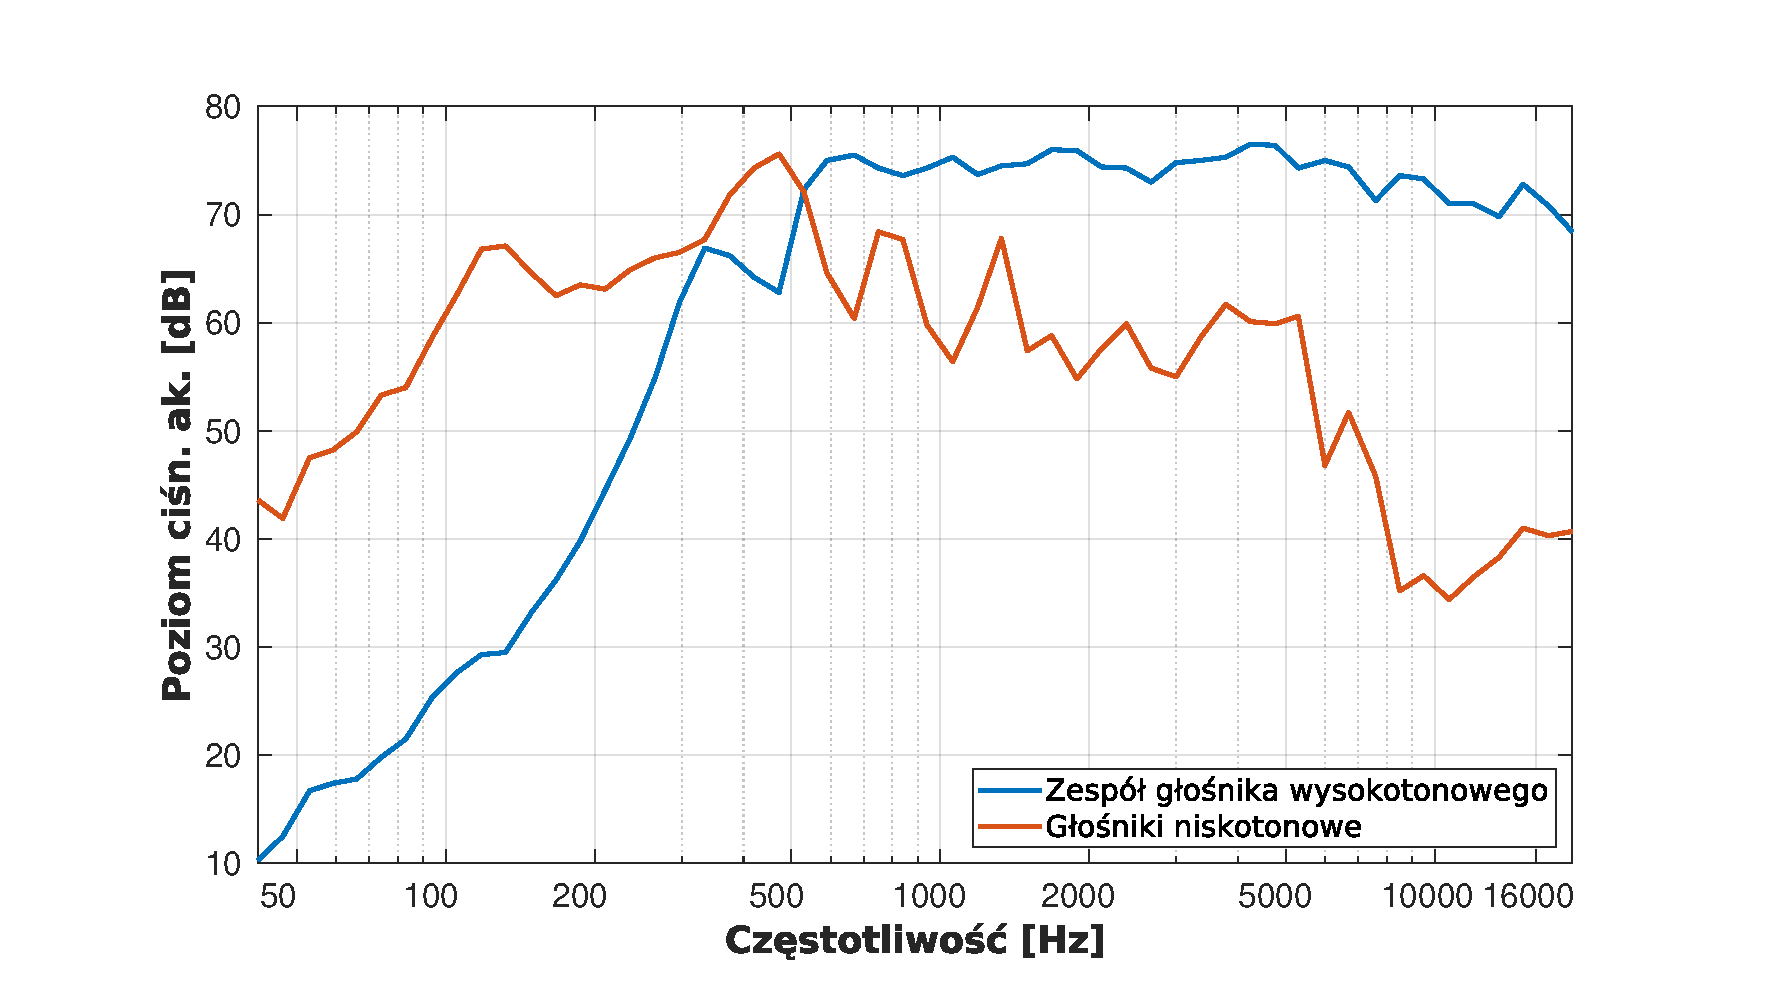
\includegraphics[width=.8\textwidth,trim={2cm .5cm 2cm 1cm},clip]{stolik_skutecznosci.pdf}
		\caption{Charakterystyki amplitudowe-częstotliwościowe badanego zestawu}
		\label{r:skutecznosc}
	\end{figure}
	
	\begin{figure}[!ht]
		\centering
		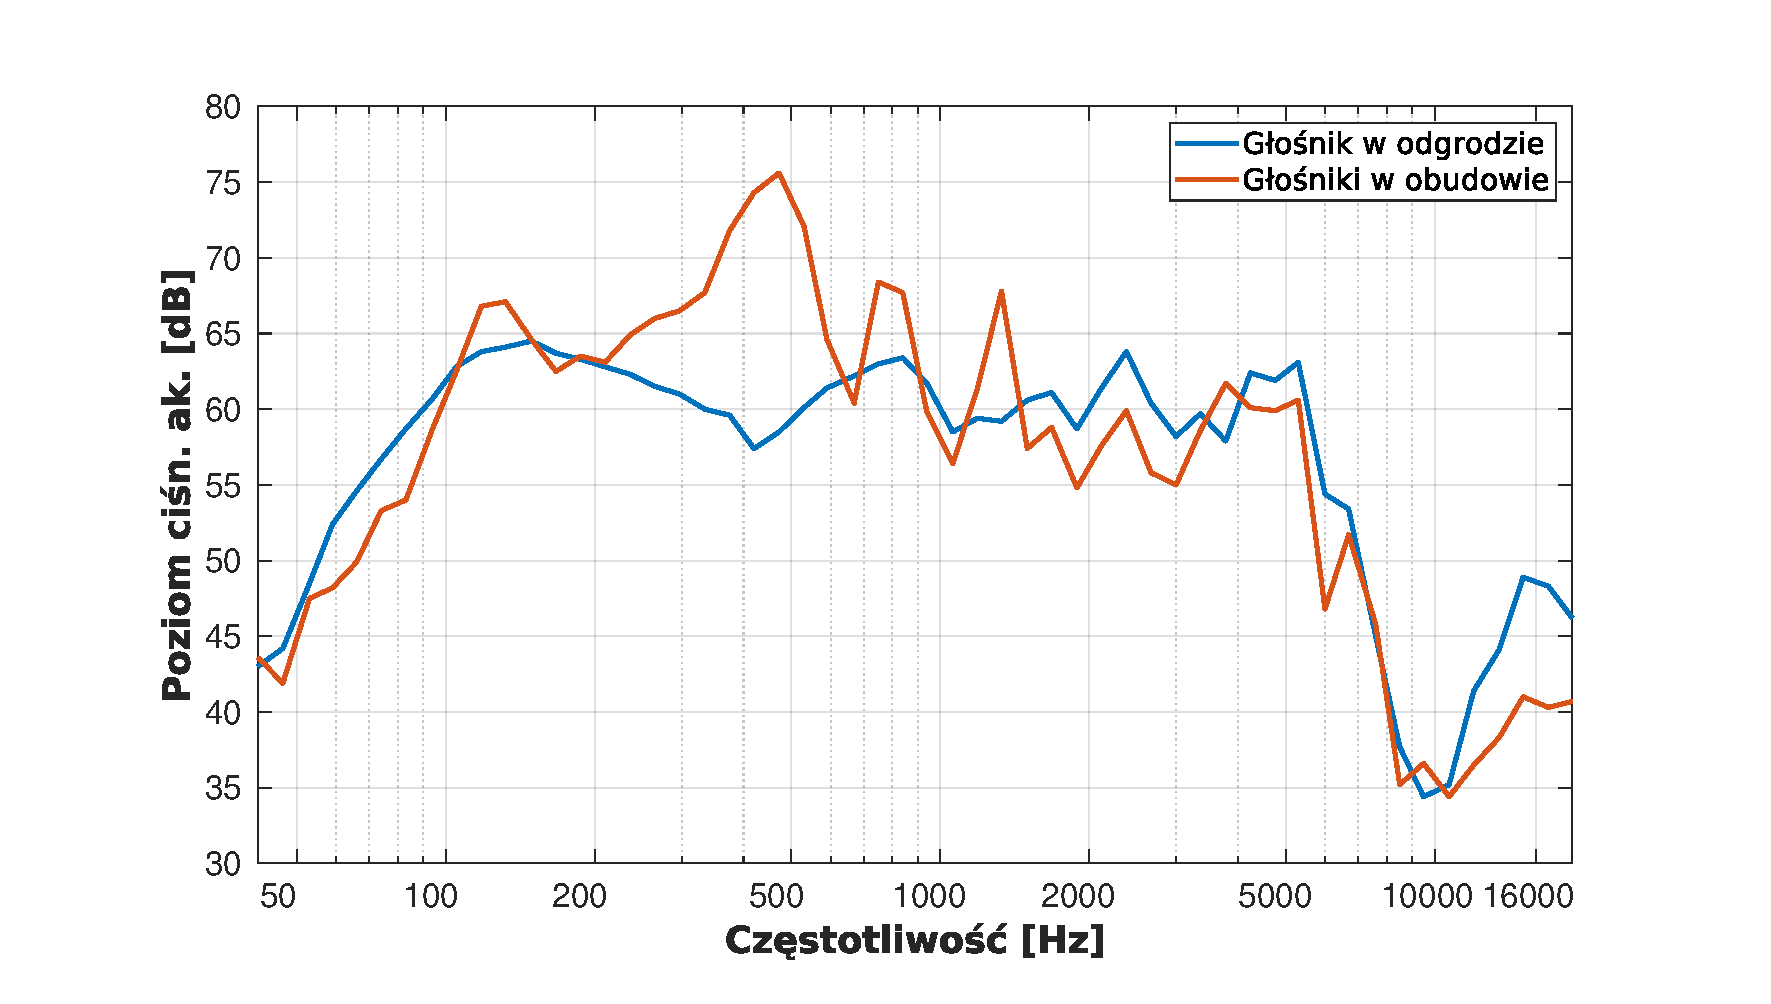
\includegraphics[width=.8\textwidth,trim={2cm .5cm 2cm 1cm},clip]{stolik_obudowa_odgroda.pdf}
		\caption{Charakterystyki amplitudowe-częstotliwościowe głośników niskotonowych w~obudowie i~głośnika w~odgrodzie}
		\label{r:skutecznosc_odgr}
	\end{figure}
	
	Dla głośników niskotonowych umieszczonych w~obudowie widoczna jest znaczącą nierównomierność charakterystyki w~zakresie \SI{490}{\hertz}. która nie jest widoczna w~charakterystyce głośnika w~odgrodzie. Należy więc przypuszczać, że wprowadza ją obudowa w~obecnej postaci; wymagane jest rozwiązanie tego problemu.
	
	\subsection{Charakterystyki kierunkowości} \label{ss:wyniki_kier}
	
	Otrzymane charakterystyki kierunkowości dla głośnika niskotonowego przedstawiono na rysunku~\ref{r:kierunkowosc_L}, a~dla zespołu głośnika wysokotonowego na rysunku~\ref{r:kierunkowosc_H}. 
	
	\begin{figure}[!ht]
		\centering
		\begin{subfigure}[b]{.52\textwidth}
			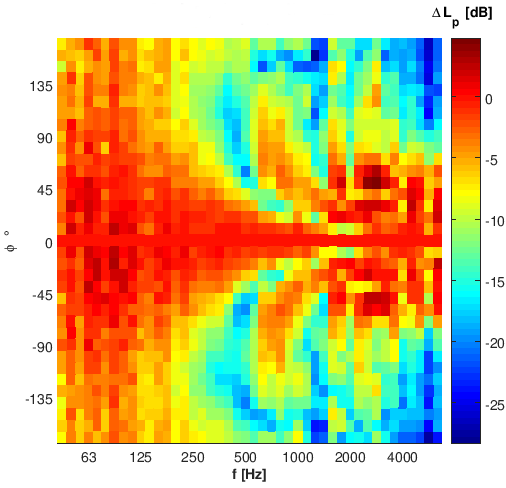
\includegraphics[width=\textwidth]{poziom_L.png}
			\caption{Płaszczyzna pozioma}
			\label{r:L_poziom}
		\end{subfigure}
		~
		\begin{subfigure}[b]{.46\textwidth}
			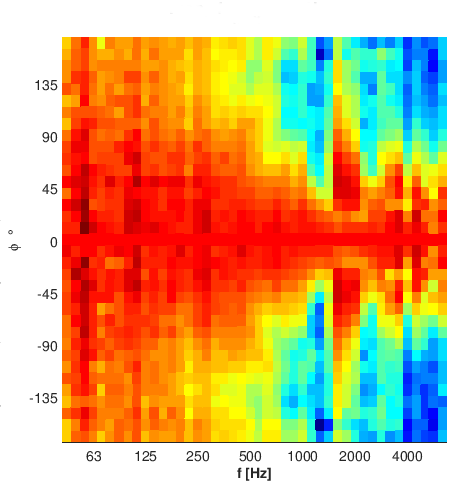
\includegraphics[width=\textwidth]{pion_L.png}
			\caption{Płaszczyzna pionowa}
			\label{r:L_pion}
		\end{subfigure}
		\caption{Charakterystyki kierunkowości głośnika niskotonowego w~obudowie}
		\label{r:kierunkowosc_L}
	\end{figure}
	
	Ze względu na kształt obudowy, kąt promieniowania głośnika niskotonowego w~płaszczyźnie pionowej jest większy, niż w~płaszczyźnie poziomej -- jest to widoczne dla pasma \range{250}{1000}~\si{\hertz}. Widoczne są też niepożądane listki boczne w~paśmie \SI{2000}{\hertz}.
	
	\begin{figure}[!ht]
		\centering
		\begin{subfigure}[b]{.52\textwidth}
			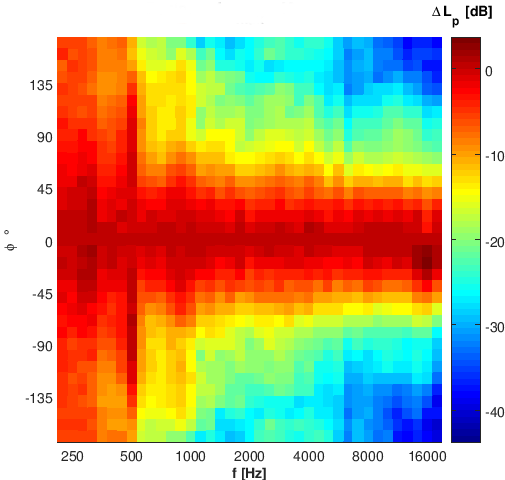
\includegraphics[width=\textwidth]{poziom_H.png}
			\caption{Płaszczyzna pozioma}
			\label{r:H_poziom}
		\end{subfigure}
		~
		\begin{subfigure}[b]{.46\textwidth}
			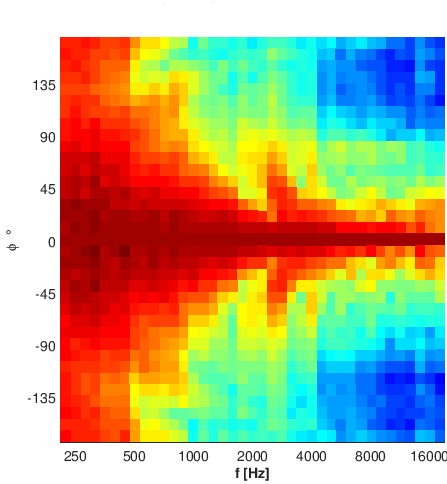
\includegraphics[width=\textwidth]{pion_H.png}
			\caption{Płaszczyzna pionowa}
			\label{r:H_pion}
		\end{subfigure}
		\caption{Charakterystyki kierunkowości zespołu głośnika wysokotonowego w~obudowie}
		\label{r:kierunkowosc_H}
	\end{figure}
	
	Z~kolei głośnik wysokotonowy charakteryzuje się bardzo równomierną charakterystyką kierunkową w~płaszczyźnie poziomej powyżej częstotliwości około \SI{1000}{Hz}.
	
	
	
	\subsection{Drgania obudowy}
	
	Analiza uzyskanych wyników nie dała podstaw do sformułowania zależności między obudową, a~charakterystykami amplitudowymi -- pomiędzy widmami sygnału z~wibrometru i~mikrofonów nie widać wyraźnych zależności. W~niektórych punktach pomiarowych można zauważyć zmiany kształtu charakterystyki dla tej samej częstotliwości, jednak są to raczej jednostkowe przypadki, na podstawie których nie można potwierdzić znaczącego wpływu na charakterystykę częstotliwościową zestawu.
	
	Spośród zarejestrowanych przebiegów wybrano punkty \range{1}{4}, między którymi można dostrzec pewne zależności i~zestawiono je na rysunku~\ref{r:wibrometr_1-4}. W~punktach tych wyraźnie widoczny jest wzrost amplitudy przemieszczeń bocznej płyty obudowy w~paśmie \SI{260}{\hertz}; jednocześnie w~tym samym paśmie zauważalny jest spadek poziomu ciśnienia akustycznego w~bliskim otoczeniu punktu (\range{6}{10}~\si{\cm}).
	
	\begin{figure}[!ht]
		\centering
		\adjincludegraphics[width=.8\textwidth,trim={2cm .5cm 2cm 1cm},clip]{pkt1_4.pdf}
		\caption{Znormalizowane widma amplitudy przemieszczeń obudowy (góra) oraz poziomu ciśnienia akustycznego (dół) w~niewielkiej odległości od zestawu w~punktach pomiarowych~\range{1}{4}}
		\label{r:wibrometr_1-4}
	\end{figure}
	
	Wybrane punkty zlokalizowane są na dwóch różnych ściankach obudowy, jak pokazano na rysunku~\ref{r:wibro_pkt}; mimo tego maksimum amplitudy drgań przypada we wszystkich czterech punktach dokładnie dla tej samej częstotliwości. Analiza częstotliwości własnych przestrzeni powietrznej wewnątrz obudowy nie daje możliwości wskazania przyczyny takiego stanu; niezbędna staje się analiza częstotliwości drgań własnych obudowy. Nie jest to jednak wada która wpływa na charakterystykę częstotliwościową zestawu, co zostało potwierdzone poprzez pomiar mikrofonem w~odległości \SI{2}{\metre}.
	
	\begin{figure}[!ht]
		\centering
		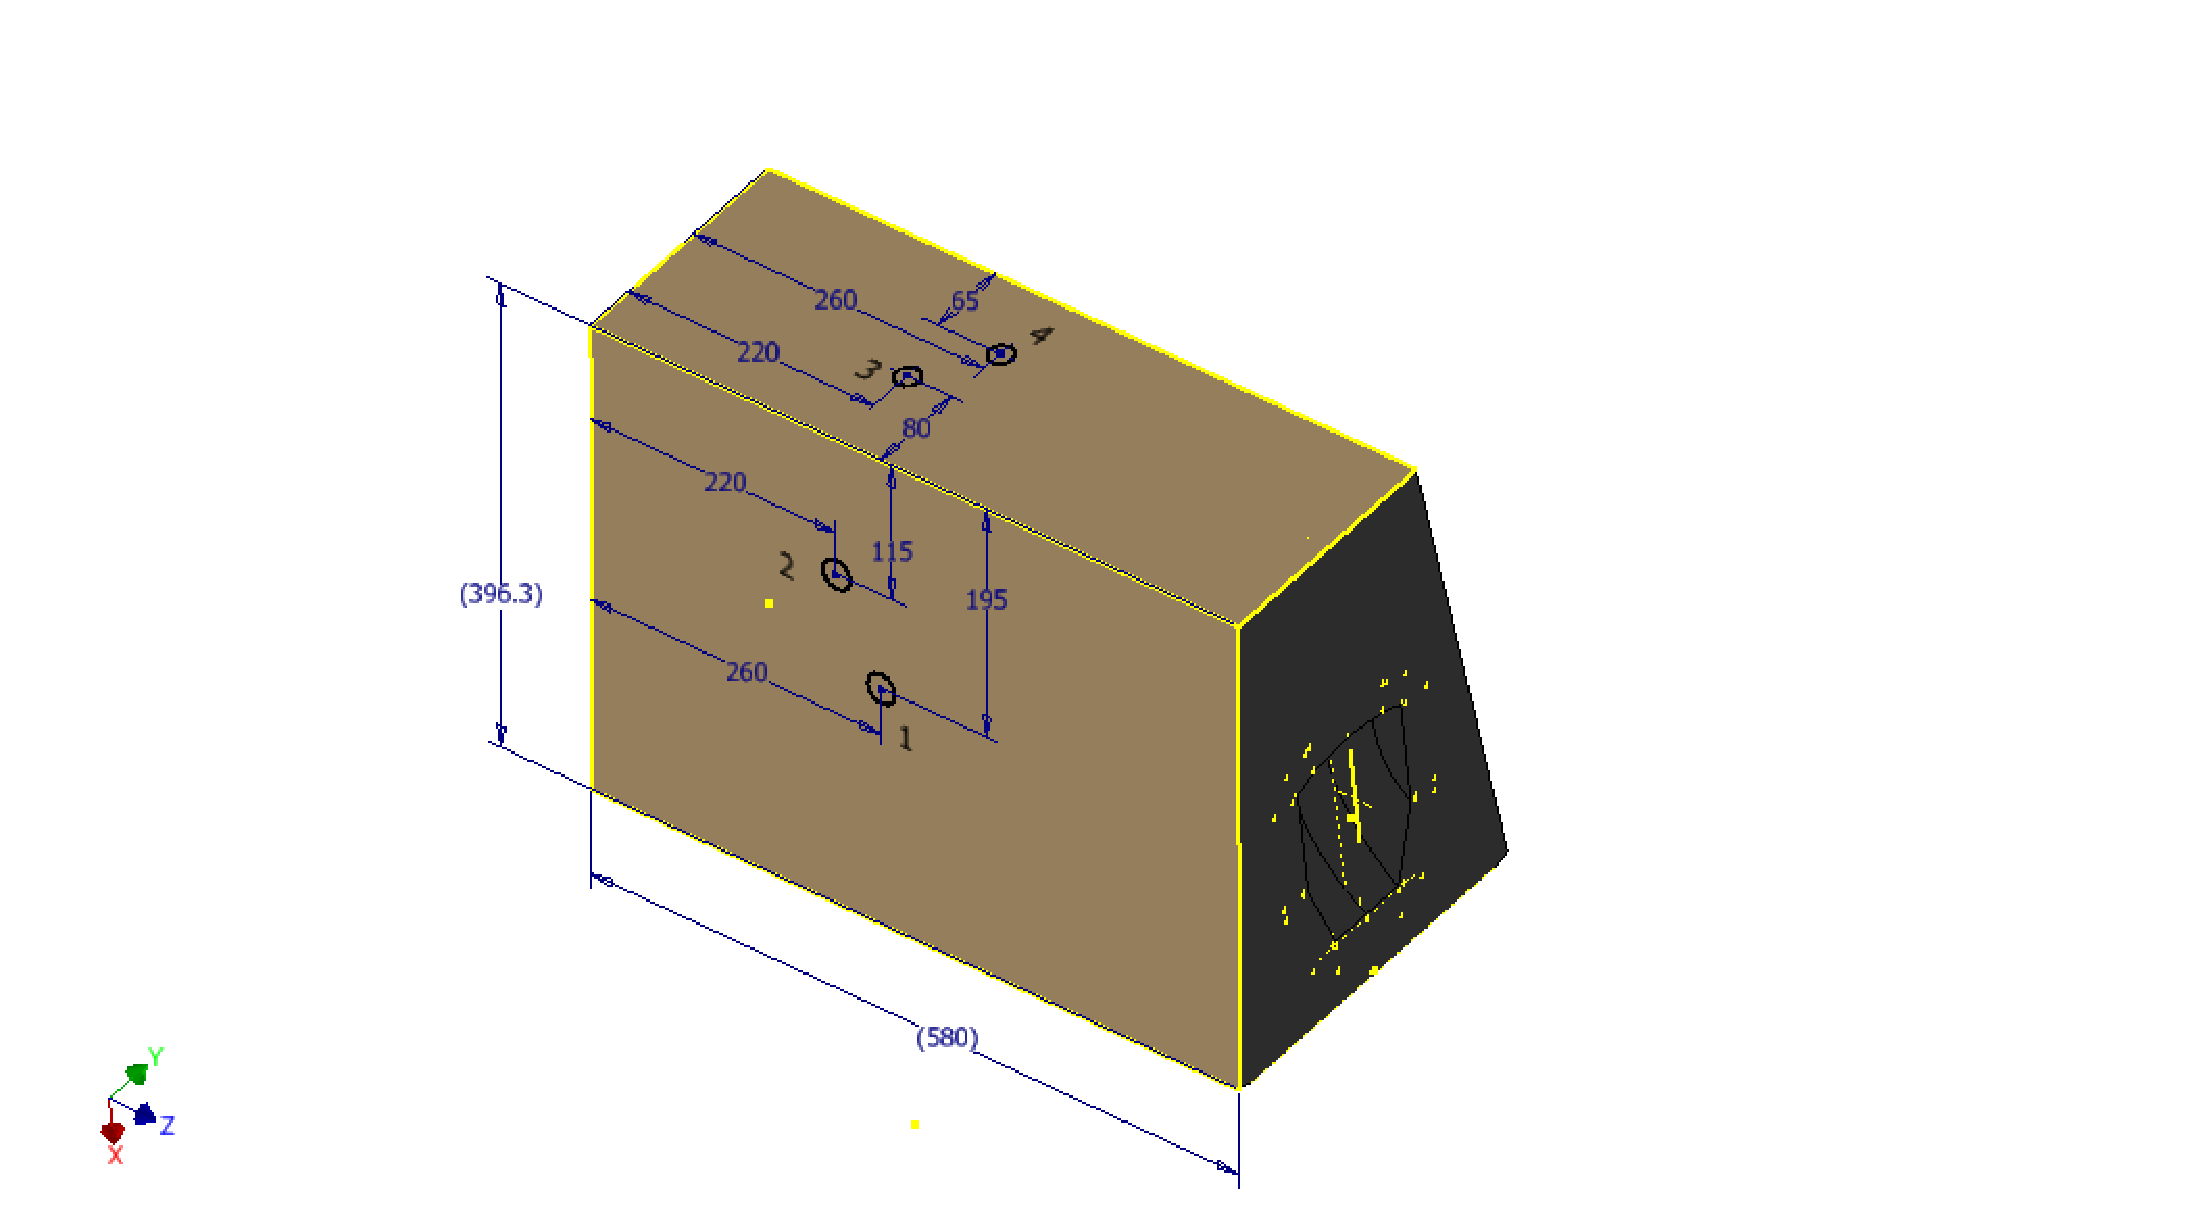
\includegraphics[width=.8\textwidth,trim={5cm .3cm 5cm 2.7cm},clip]{wibrometr.pdf}
		\caption{Rozmieszczenie punktów pomiarowych \range{1}{4} na obudowie (widok tylnej i~górnej ścianki)}
		\label{r:wibro_pkt}
	\end{figure}
	
	Kolejnym punktem, dla którego zdecydowano się zaprezentować wyniki jest punkt~\num{5}, zlokalizowany na powierzchni wnęki uchwytu (na rysunku~\ref{r:wibro_pkt} po prawej stronie). Na widmie przemieszczeń (rysunek~\ref{r:wibrometr_5}) widoczne jest lokalne maksimum amplitudy dla częstotliwości~\SI{400}{\hertz}, co jednak nie znajduje odzwierciedlenia w~widmie poziomu ciśnienia akustycznego -- mimo że podbicie tej częstotliwości jest widoczne w~charakterystykach skuteczności (por. rys.~\ref{r:skutecznosc}).%Drgania obudowy mogą mieć wpływ na pole akustyczne wokół zestawu.
	
	\begin{figure}[H]
		\centering
		\adjincludegraphics[width=.8\textwidth,trim={2cm .5cm 2cm 1cm},clip]{pkt5.pdf}
		\caption{Znormalizowane widma amplitudy przemieszczeń obudowy (góra) oraz poziomu ciśnienia akustycznego w~niewielkiej odległości od zestawu w~punkcie pomiarowym~\num{5}}
		\label{r:wibrometr_5}
	\end{figure}
	
	Otrzymane wyniki nie dają podstaw do jednoznacznego wskazania wpływu drgań obudowy na charakterystykę częstotliwościową zestawu. Jednocześnie do dalszej analizy tej zależności wskazane jest wykonanie pomiarów w~większej liczbie punktów oraz obliczeń statystycznych.
	
	\subsection{Symulacje numeryczne}
	
	Dla wstępnie dostrojonego modelu przeprowadzono symulacje rozkładu ciśnienia akustycznego wokół zestawu oraz przemieszczenia membrany. Wyznaczono także charakterystykę skuteczności zestawu. 
	
	Na rysunku~\ref{r:C_rozklady} przedstawiono rozkłady ciśnienia akustycznego w~zestawieniu ze skutecznością zestawu. Podbicie charakterystyki w~okolicach \SI{500}{\hertz} znajduje odzwierciedlenie na rysunkach~\ref{r:C_500} i~\ref{r:C_560} -- fale dźwiękowe nakładają się w~taki sposób, że możliwa jest ich dalsza propagacja. Natomiast dla częstotliwości \SI{710}{\hertz}, dla której w~charakterystyce skuteczności widoczny jest nagły spadek, występuje zjawisko zwarcia akustycznego: głośnik i~otwór \textit{bass-reflex} emitują fale w~przeciwfazie, które wygaszają się wzajemnie przed głośnikiem (rysunek~\ref{r:C_710}). Można to zauważyć na rysunku~\ref{r:C_balony}, który przedstawia linie jednakowego ciśnienia wokół zestawu.
	
	\begin{figure}[!ht]
		\centering
		\begin{subfigure}[b]{.49\textwidth}
			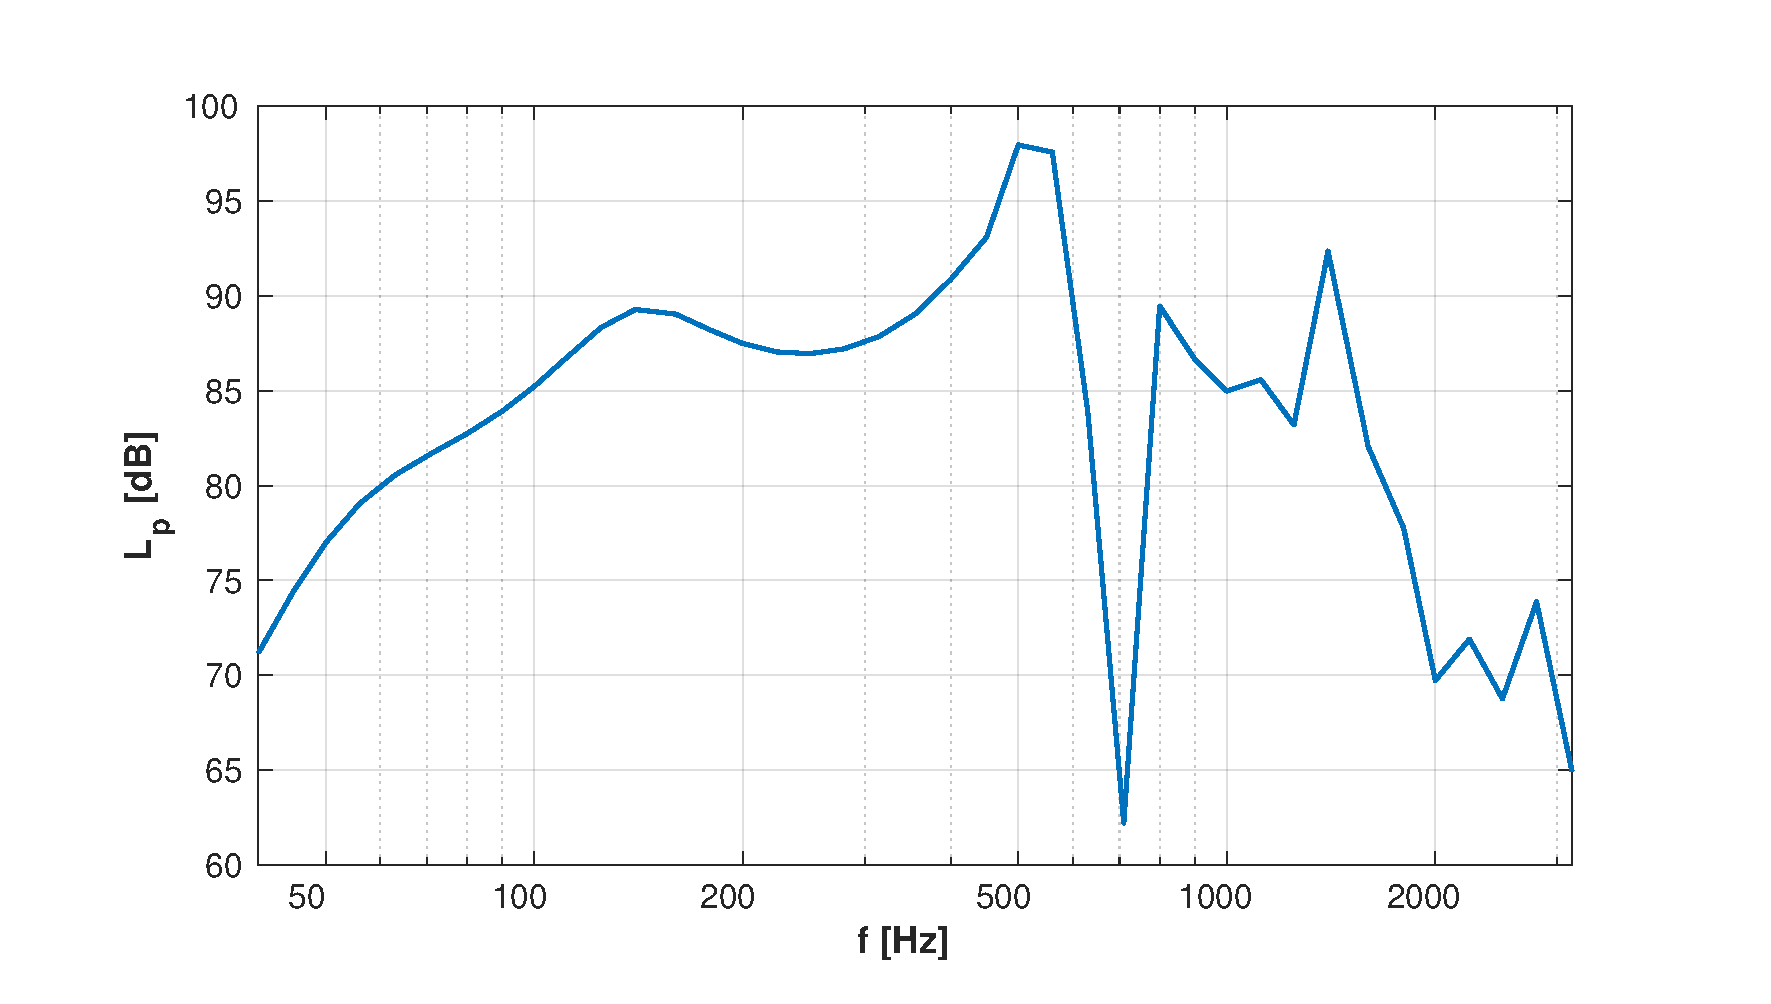
\includegraphics[width=\textwidth,trim={1.25cm .5cm 2cm 1cm},clip]{skutecznosc_comsol.pdf}
			\caption{Skuteczność zestawu}
			\label{r:C_skutecznosc}
		\end{subfigure}
		~
		\begin{subfigure}[b]{.49\textwidth}
			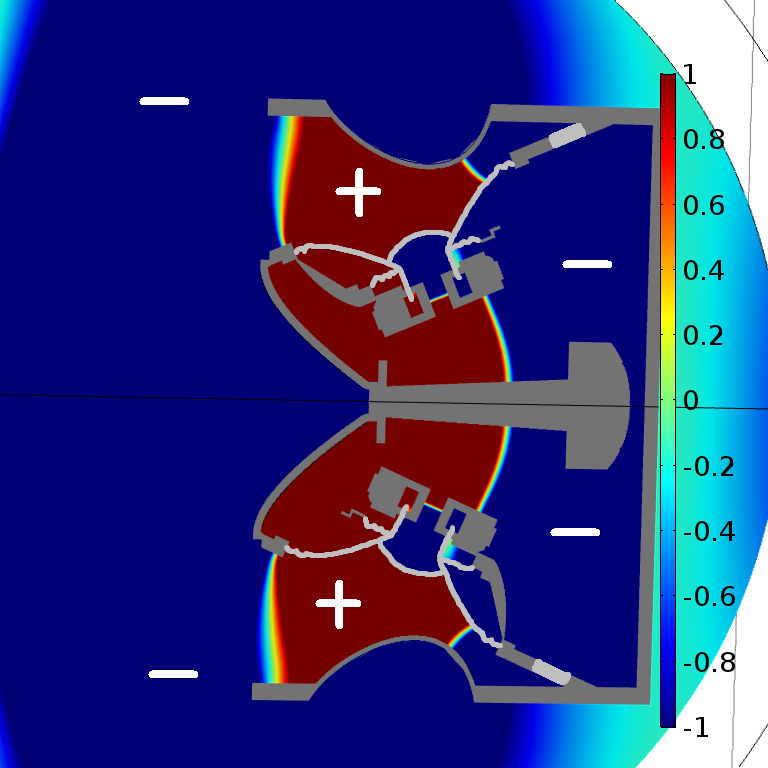
\includegraphics[width=\textwidth]{pres_sig_500Hz_02.png}
			\caption{Rozkład ciśnienia akustycznego dla częstotliwości \SI{500}{\hertz}}
			\label{r:C_500}
		\end{subfigure}
		
		\begin{subfigure}[b]{.49\textwidth}
			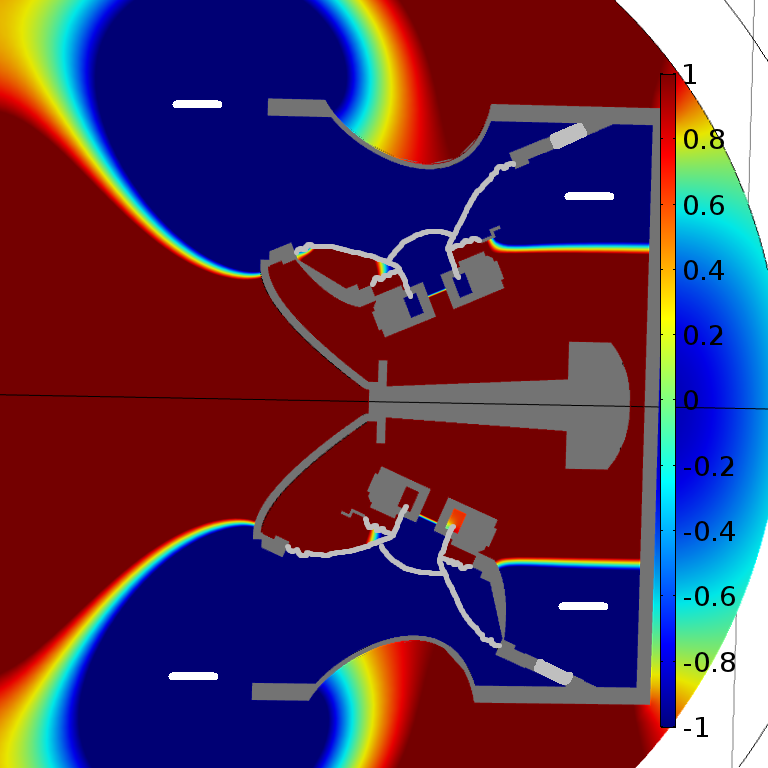
\includegraphics[width=\textwidth]{pres_sig_560Hz_02.png}
			\caption{Rozkład ciśnienia akustycznego dla częstotliwości \SI{560}{\hertz}}
			\label{r:C_560}
		\end{subfigure}
		~
		\begin{subfigure}[b]{.49\textwidth}
			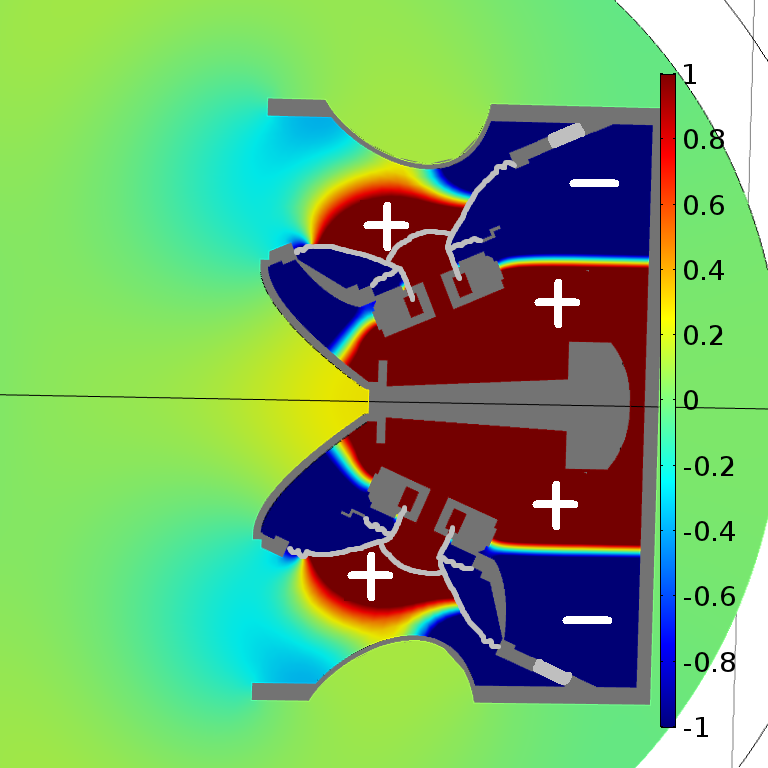
\includegraphics[width=\textwidth]{pres_sig_710Hz_02.png}
			\caption{Rozkład ciśnienia akustycznego dla częstotliwości \SI{710}{\hertz}}
			\label{r:C_710}
		\end{subfigure}
		% 			\caption{Wyniki uzyskane z~symulacji w~środowisku Comsol; dla rozkładów ciśnienia wartości powyżej \SI{1}{\pascal} i~poniżej \SI{-1}{\pascal} zostały zaokrąglone do tych wartości dla zwiększenia czytelności}
		\caption{Wyniki uzyskane z~symulacji w~środowisku Comsol; dla rozkładów ciśnienia skala wyświetlania została zawężona do zakresu $[-1;1]$~\si{\pascal} w~celu zwiększenia czytelności}
		\label{r:C_rozklady}
	\end{figure}
	
	\begin{figure}[!ht]
		\centering
		\begin{subfigure}[b]{.49\textwidth}
			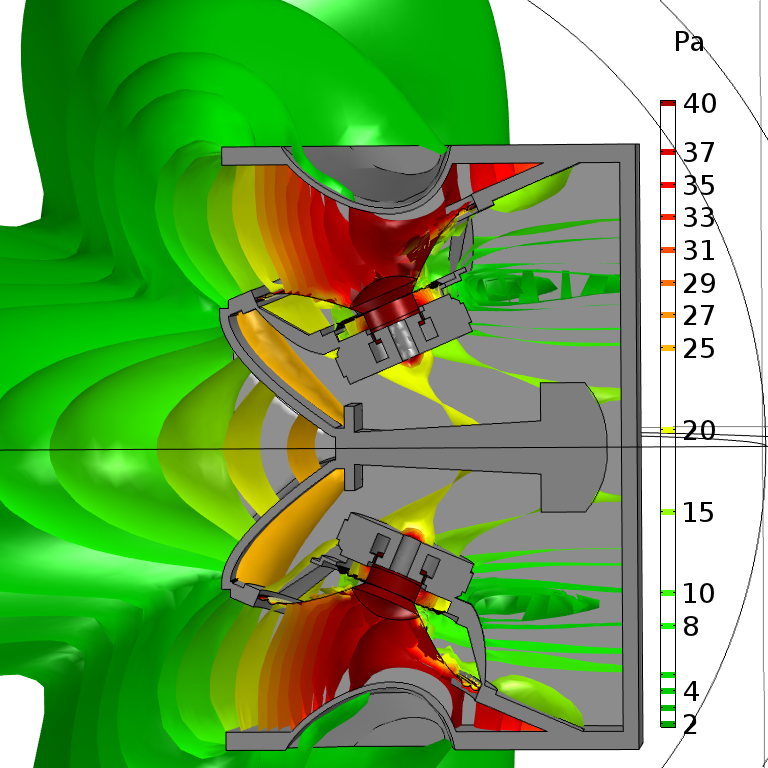
\includegraphics[width=\textwidth]{absp_560Hz.png}
			\caption{Częstotliwość \SI{560}{\hertz}}
			\label{r:C_560iz}
		\end{subfigure}
		~
		\begin{subfigure}[b]{.49\textwidth}
			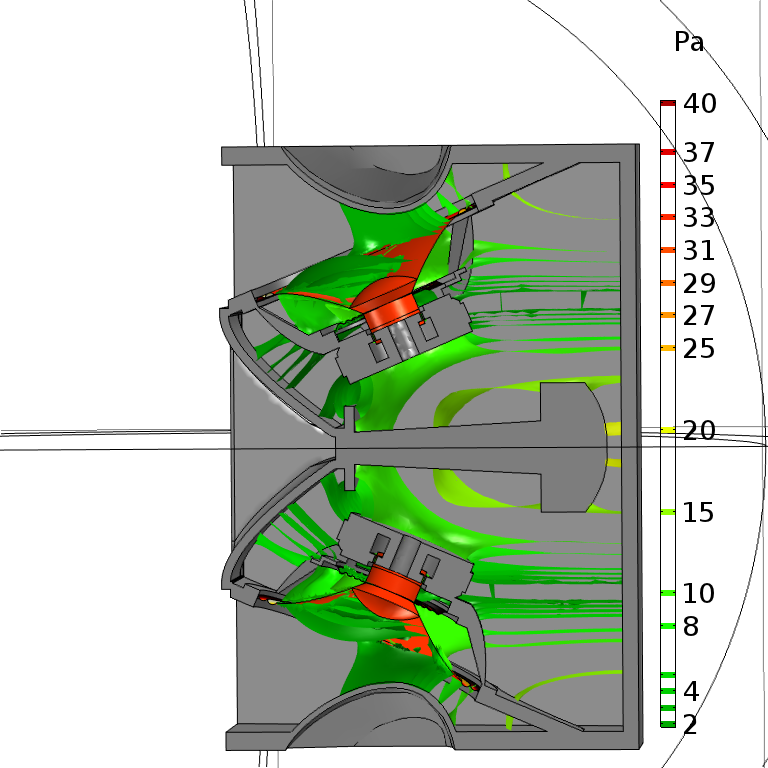
\includegraphics[width=\textwidth]{absp_710Hz.png}
			\caption{Częstotliwość \SI{710}{\hertz}}
			\label{r:C_710iz}
		\end{subfigure}
		
		\caption{Izobary uzyskane z~symulacji w~środowisku Comsol}
		\label{r:C_balony}
	\end{figure}
	
	Rysunek \ref{r:C_przem_cisn} przedstawia kolejną z~przydatnych funkcjonalności jaką daje model zestawu głośnikowego analizowany metodą elementów skończonych: dzięki możliwości sprzężenia domen możliwa stała się szybka i~łatwa obserwacja odkształceń zawieszenia górnego głośnika. 
	
	Zastosowany układ zestawu powoduje nierównomierne obciążenie membrany głośnika i~wspomnianego zawieszenia. W obszarze blisko frontowej części zestawu (górna część ilustracji) zawieszenie znajduje się pomiędzy obszarami o~przeciwnych wartościach ciśnienia akustycznego, dokładnie odwrotnie niż ma to miejsce w~wewnętrznej części zestawu. Tam różnica ciśnień akustycznych rozdzielonych zawieszeniem i membraną jest dużo mniejsza. Występowanie na obwodzie nierównomierności tego typu powoduje osiowo niesymetryczne ruchu membrany, przez to zwiększając poziom zniekształceń; niesymetryczne obciążenie zawieszenia może przyczyniać się do jego szybszego zużycia, a~w~konsekwencji do awarii przetwornika.  
	
	\begin{figure}[!ht]
		\centering
		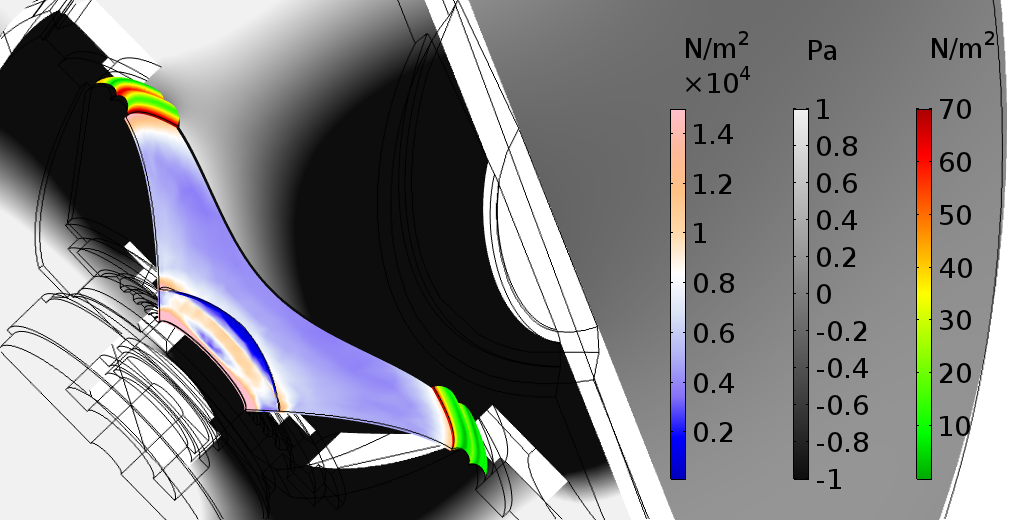
\includegraphics[width=\textwidth]{stress_pressure_1kHz.png}
		\caption{Naprężenia na membranie i~zawieszeniu i~rozkład ciśnienia akustycznego (ciemne obszary oznaczają ujemne ciśnienie, jasne -- dodatnie)}
		\label{r:C_przem_cisn}
	\end{figure}
	
	Oprócz rozkładu ciśnienia w~przestrzeni wyznaczono także charakterystyki kierunkowości (rysunek~\ref{r:C_kierunk}). Porównując ich kształt z~wynikami pomiarów (por. część~\ref{ss:wyniki_kier}) można zauważyć duże podobieństwo, zwłaszcza w~płaszczyźnie poziomej.
	
	\begin{figure}[!ht]
		\centering
		\begin{subfigure}[b]{.49\textwidth}
			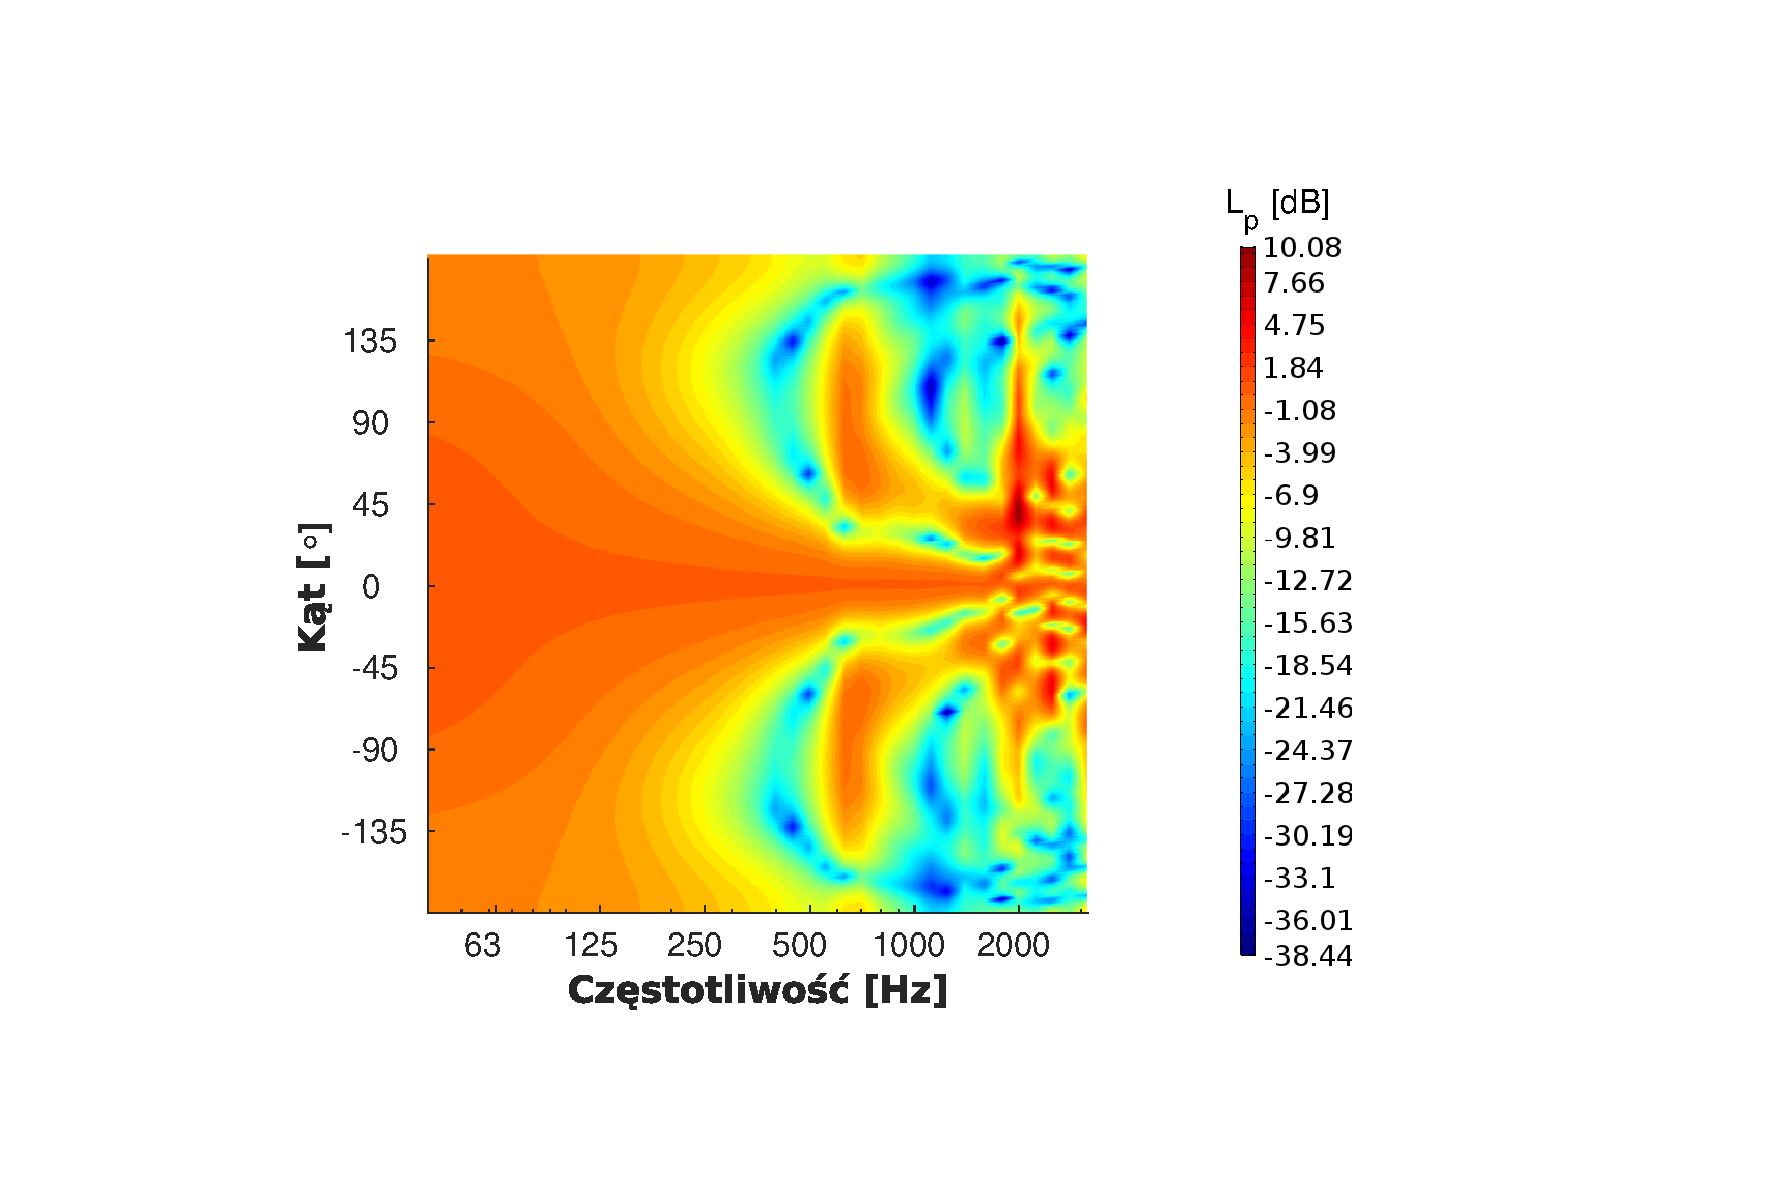
\includegraphics[width=\textwidth,trim={4.6cm 2.6cm 5.8cm 2.7cm},clip]{Comsol_kier_osie_hor.pdf}
			\caption{Płaszczyzna pozioma}
			\label{r:C_poziom}
		\end{subfigure}
		~
		\begin{subfigure}[b]{.49\textwidth}
			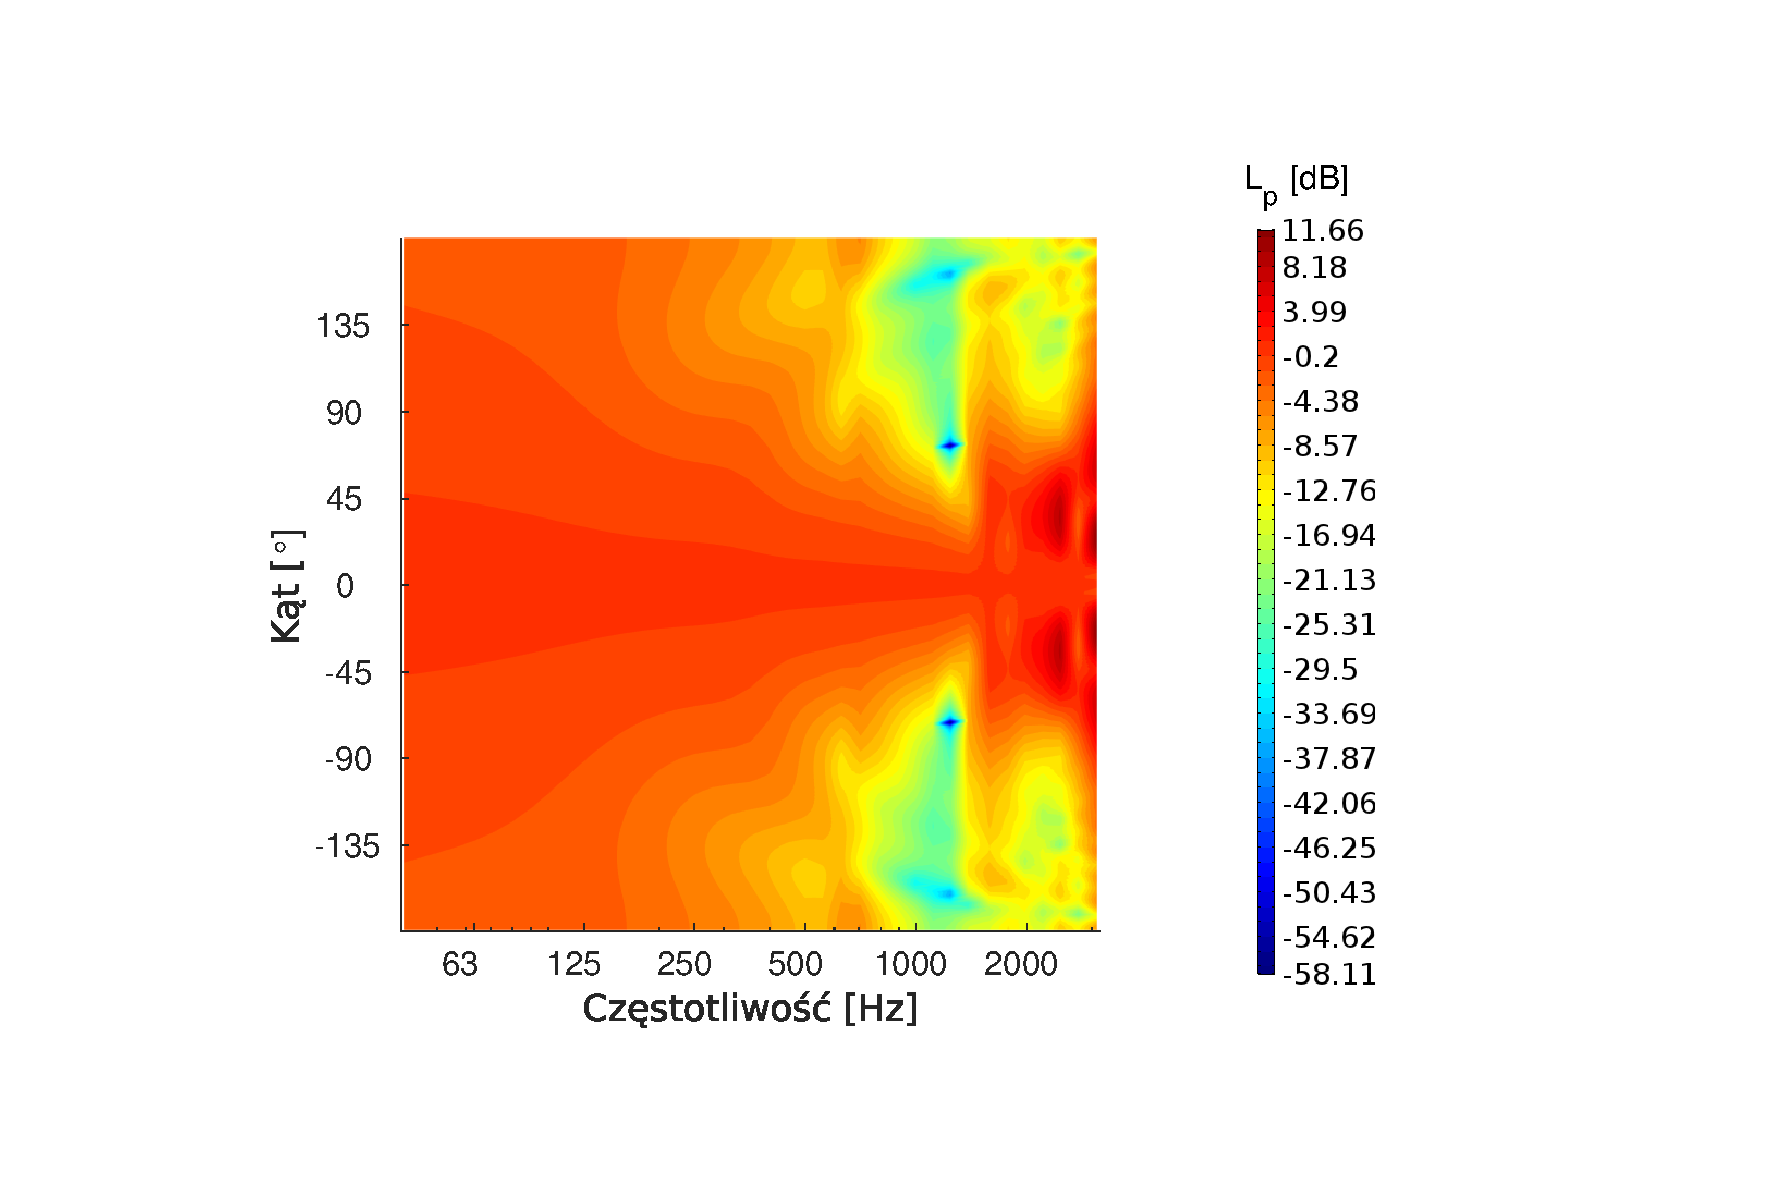
\includegraphics[width=\textwidth,trim={4.6cm 2.6cm 5.8cm 2.7cm},clip]{Comsol_kier_osie_ver.pdf}
			\caption{Płaszczyzna pionowa}
			\label{r:C_pion}
		\end{subfigure}
		
		\caption{Charakterystyki kierunkowości uzyskane z~symulacji w~środowisku Comsol}
		\label{r:C_kierunk}
	\end{figure}
	
	\section{Podsumowanie}
	
	Otrzymane dotychczas wyniki wskazują, iż optymalnym byłoby przyjęcie częstotliwości granicznych dla głośnika wysoko- i niskotonowego w~przedziale ~\range{1000}{1200}\si{Hz}. Wymaga to jednak uwzględnienia charakterystyki fazowej głośników niskotonowych i zespołu głośnika wysokotonowego w~obudowie, po zastosowaniu możliwych rozwiązań poprawiających charakterystykę amplitudowo-częstotliwościową w~zakresie przetwarzanym przez głośniki niskotonowe. 
	
	Planowane jest wykonanie kolejnych pomiarów, obejmujących inne modyfikacje obudowy, mających na celu poprawę charakterystyki amplitudowo-częstotliwościowej oraz równomierności charakterystyk kierunkowości. 
	
	Autorzy pracują także nad dostrojeniem modelu komputerowego, aby móc prowadzić dalsze badania na drodze symulacji. Pozwoliłoby to na określenie wpływu poszczególnych elementów konstrukcji na charakterystyki zestawu oraz rozwój wiedzy i~umiejętności, które mogą zostać wykorzystane do budowy zestawu od podstaw. 
	
	\printbibliography
	
\end{document}
